% Options for packages loaded elsewhere
\PassOptionsToPackage{unicode}{hyperref}
\PassOptionsToPackage{hyphens}{url}
%
\documentclass[
]{article}
\usepackage{amsmath,amssymb}
\usepackage{iftex}
\ifPDFTeX
  \usepackage[T1]{fontenc}
  \usepackage[utf8]{inputenc}
  \usepackage{textcomp} % provide euro and other symbols
\else % if luatex or xetex
  \usepackage{unicode-math} % this also loads fontspec
  \defaultfontfeatures{Scale=MatchLowercase}
  \defaultfontfeatures[\rmfamily]{Ligatures=TeX,Scale=1}
\fi
\usepackage{lmodern}
\ifPDFTeX\else
  % xetex/luatex font selection
\fi
% Use upquote if available, for straight quotes in verbatim environments
\IfFileExists{upquote.sty}{\usepackage{upquote}}{}
\IfFileExists{microtype.sty}{% use microtype if available
  \usepackage[]{microtype}
  \UseMicrotypeSet[protrusion]{basicmath} % disable protrusion for tt fonts
}{}
\makeatletter
\@ifundefined{KOMAClassName}{% if non-KOMA class
  \IfFileExists{parskip.sty}{%
    \usepackage{parskip}
  }{% else
    \setlength{\parindent}{0pt}
    \setlength{\parskip}{6pt plus 2pt minus 1pt}}
}{% if KOMA class
  \KOMAoptions{parskip=half}}
\makeatother
\usepackage{xcolor}
\usepackage[margin=1in]{geometry}
\usepackage{color}
\usepackage{fancyvrb}
\newcommand{\VerbBar}{|}
\newcommand{\VERB}{\Verb[commandchars=\\\{\}]}
\DefineVerbatimEnvironment{Highlighting}{Verbatim}{commandchars=\\\{\}}
% Add ',fontsize=\small' for more characters per line
\usepackage{framed}
\definecolor{shadecolor}{RGB}{248,248,248}
\newenvironment{Shaded}{\begin{snugshade}}{\end{snugshade}}
\newcommand{\AlertTok}[1]{\textcolor[rgb]{0.94,0.16,0.16}{#1}}
\newcommand{\AnnotationTok}[1]{\textcolor[rgb]{0.56,0.35,0.01}{\textbf{\textit{#1}}}}
\newcommand{\AttributeTok}[1]{\textcolor[rgb]{0.13,0.29,0.53}{#1}}
\newcommand{\BaseNTok}[1]{\textcolor[rgb]{0.00,0.00,0.81}{#1}}
\newcommand{\BuiltInTok}[1]{#1}
\newcommand{\CharTok}[1]{\textcolor[rgb]{0.31,0.60,0.02}{#1}}
\newcommand{\CommentTok}[1]{\textcolor[rgb]{0.56,0.35,0.01}{\textit{#1}}}
\newcommand{\CommentVarTok}[1]{\textcolor[rgb]{0.56,0.35,0.01}{\textbf{\textit{#1}}}}
\newcommand{\ConstantTok}[1]{\textcolor[rgb]{0.56,0.35,0.01}{#1}}
\newcommand{\ControlFlowTok}[1]{\textcolor[rgb]{0.13,0.29,0.53}{\textbf{#1}}}
\newcommand{\DataTypeTok}[1]{\textcolor[rgb]{0.13,0.29,0.53}{#1}}
\newcommand{\DecValTok}[1]{\textcolor[rgb]{0.00,0.00,0.81}{#1}}
\newcommand{\DocumentationTok}[1]{\textcolor[rgb]{0.56,0.35,0.01}{\textbf{\textit{#1}}}}
\newcommand{\ErrorTok}[1]{\textcolor[rgb]{0.64,0.00,0.00}{\textbf{#1}}}
\newcommand{\ExtensionTok}[1]{#1}
\newcommand{\FloatTok}[1]{\textcolor[rgb]{0.00,0.00,0.81}{#1}}
\newcommand{\FunctionTok}[1]{\textcolor[rgb]{0.13,0.29,0.53}{\textbf{#1}}}
\newcommand{\ImportTok}[1]{#1}
\newcommand{\InformationTok}[1]{\textcolor[rgb]{0.56,0.35,0.01}{\textbf{\textit{#1}}}}
\newcommand{\KeywordTok}[1]{\textcolor[rgb]{0.13,0.29,0.53}{\textbf{#1}}}
\newcommand{\NormalTok}[1]{#1}
\newcommand{\OperatorTok}[1]{\textcolor[rgb]{0.81,0.36,0.00}{\textbf{#1}}}
\newcommand{\OtherTok}[1]{\textcolor[rgb]{0.56,0.35,0.01}{#1}}
\newcommand{\PreprocessorTok}[1]{\textcolor[rgb]{0.56,0.35,0.01}{\textit{#1}}}
\newcommand{\RegionMarkerTok}[1]{#1}
\newcommand{\SpecialCharTok}[1]{\textcolor[rgb]{0.81,0.36,0.00}{\textbf{#1}}}
\newcommand{\SpecialStringTok}[1]{\textcolor[rgb]{0.31,0.60,0.02}{#1}}
\newcommand{\StringTok}[1]{\textcolor[rgb]{0.31,0.60,0.02}{#1}}
\newcommand{\VariableTok}[1]{\textcolor[rgb]{0.00,0.00,0.00}{#1}}
\newcommand{\VerbatimStringTok}[1]{\textcolor[rgb]{0.31,0.60,0.02}{#1}}
\newcommand{\WarningTok}[1]{\textcolor[rgb]{0.56,0.35,0.01}{\textbf{\textit{#1}}}}
\usepackage{longtable,booktabs,array}
\usepackage{calc} % for calculating minipage widths
% Correct order of tables after \paragraph or \subparagraph
\usepackage{etoolbox}
\makeatletter
\patchcmd\longtable{\par}{\if@noskipsec\mbox{}\fi\par}{}{}
\makeatother
% Allow footnotes in longtable head/foot
\IfFileExists{footnotehyper.sty}{\usepackage{footnotehyper}}{\usepackage{footnote}}
\makesavenoteenv{longtable}
\usepackage{graphicx}
\makeatletter
\def\maxwidth{\ifdim\Gin@nat@width>\linewidth\linewidth\else\Gin@nat@width\fi}
\def\maxheight{\ifdim\Gin@nat@height>\textheight\textheight\else\Gin@nat@height\fi}
\makeatother
% Scale images if necessary, so that they will not overflow the page
% margins by default, and it is still possible to overwrite the defaults
% using explicit options in \includegraphics[width, height, ...]{}
\setkeys{Gin}{width=\maxwidth,height=\maxheight,keepaspectratio}
% Set default figure placement to htbp
\makeatletter
\def\fps@figure{htbp}
\makeatother
\setlength{\emergencystretch}{3em} % prevent overfull lines
\providecommand{\tightlist}{%
  \setlength{\itemsep}{0pt}\setlength{\parskip}{0pt}}
\setcounter{secnumdepth}{-\maxdimen} % remove section numbering
\ifLuaTeX
  \usepackage{selnolig}  % disable illegal ligatures
\fi
\IfFileExists{bookmark.sty}{\usepackage{bookmark}}{\usepackage{hyperref}}
\IfFileExists{xurl.sty}{\usepackage{xurl}}{} % add URL line breaks if available
\urlstyle{same}
\hypersetup{
  pdftitle={Hooge Raam open water with groundwater interactions},
  hidelinks,
  pdfcreator={LaTeX via pandoc}}

\title{Hooge Raam open water with groundwater interactions}
\author{}
\date{\vspace{-2.5em}}

\begin{document}
\maketitle

{
\setcounter{tocdepth}{2}
\tableofcontents
}
\hypertarget{introduction}{%
\section{Introduction}\label{introduction}}

With this final assignment both an open water model and a groundwater
model will be developed which will be coupled.\\
De open water model represents a small river called the Hooge Raam. The
groundwater model will simulate the transition of precipitation into
drainage and surface runoff of the area surrounding the Hooge Raam.\\
Flow in the open water model is based on the diffusive wave (``Froude =
0'') approximation in 1D. Groundwater flow is based on Darcy's equation
and simulates the flow between two open water courses (ditches or
drains) in 1D. Groundwater flow will be simulated in transient mode to
account for storage changes. The open water flow model simulates in
pseudo stationary mode.\\
A storm event, a heavy rain shower, is the forcing for which we will
investigate flow from the surface into the soil, towards ditches and
finally to the Hooge Raam to get discharged at the weir on the lower
side.

The Hooge Raam is located just below the small town Grave and is part of
the water board ``Aa en Maas''. The surrounding area is mainly used as
grasslands, some cornfields and a few forest plots. The area is
reasonably flat where surface levels range from 15.5 till about 17.5 m
AMSL (Above Mean Sea Level).

The figure below gives an overview of the Hooge Raam which will be
considered for modeling.

\begin{figure}
\centering
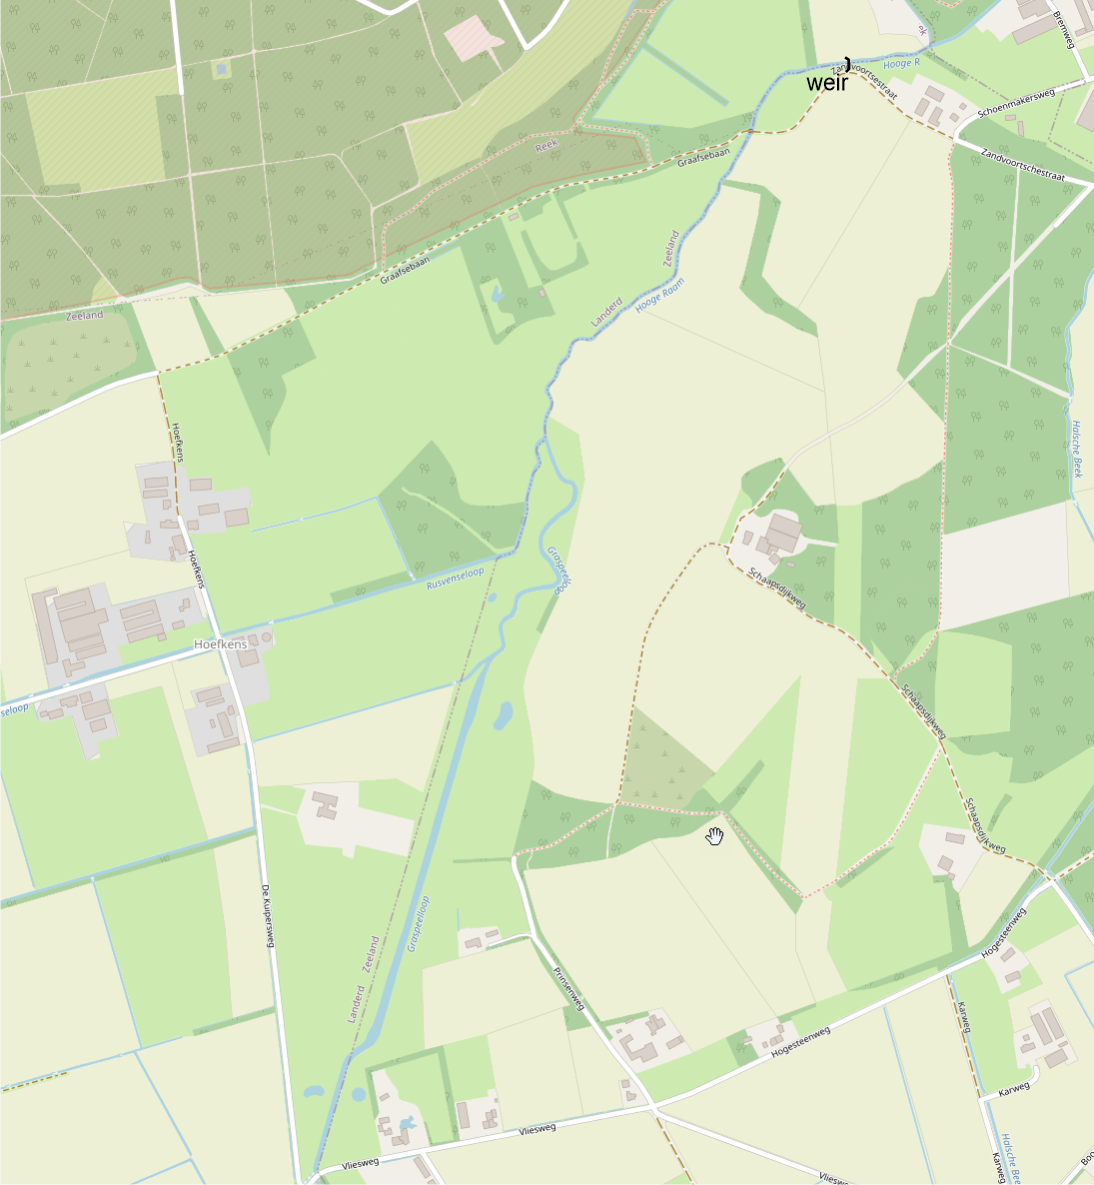
\includegraphics{Hooge-raam_overview.png}
\caption{Overview Hooge Raam and area}
\end{figure}

The first part contains the explanation and assignments for the open
water model, the second will go into the details of the groundwater
model, the coupling of both models is described in the third part and
finally the last part (4) contains the setup to determine derived
uncertainties of the ``model-train''.

\hypertarget{part-1-the-open-water-model}{%
\section{PART 1 the Open water
model}\label{part-1-the-open-water-model}}

\hypertarget{open-water-equations}{%
\subsection{Open water equations}\label{open-water-equations}}

This document should give an introduction to the hydraulic modeling of
the Hooge Raam river.

An attempt is made to make the document self contained. For that reason
we start by giving some basic formulas, and more formulas will follow
further in the document. This document should however not to be
considered as a course in hydrodynamics. The formulas are cited (which
should be for most of you a repetition?) to form the base of the code.

The flow in rivers as the Hooge Raam is most often described by the so
called St-Venant equations, expressing respectively the mass and the
momentum balance (only in \emph{x}-direction:

\[
\frac{\partial A}{\partial t} + \frac{\partial Q}{\partial x} = I\\
\frac{\partial Q}{\partial t} + \frac{\partial Q\,u}{\partial x} 
            = g\;A\;\Big( S_o - S_f - \frac{\partial a}{\partial x}\Big)
\]

As we are here less interested in highly dynamic open water
calculations, a simplification of the second equation above will be
used. This simplification starts from the observation that in many
situations (certainly lowland situations) the first two terms in the
momentum part of the St-Venant equations are much smaller than the terms
on the right hand side.

\[
\frac{\partial Q}{\partial t} + \frac{\partial Q\,u}{\partial x} = 
        g\;A\;\Big( S_o - S_f - \frac{\partial a}{\partial x}\Big)\\
\Downarrow \\
0 = g\;A\;\Big( S_o - S_f - \frac{\partial a}{\partial x}\Big)\\
\Downarrow \\
0 =  S_o - S_f - \frac{\partial a}{\partial x}
\]

The meaning of the terms in these equations will be explained when they
first appear in this document.

In these exercises situations will be studied where

\begin{itemize}
\tightlist
\item
  the flow in the Hooge Raam can be considered to be \emph{stationary}
  (so the time derivatives in the equations above disappear)
\item
  there is a weir at the downstream end of the river
\end{itemize}

Situations of this type are often called \textbf{backwater curves}.

This type of open water model that will be developed in this document
will be coupled with a groundwater model. So at some places typical
groundwater terms and dimensions may occur.

The open water has its own standard units:

\begin{itemize}
\tightlist
\item
  length unit = \(m\) meter
\item
  time unit = \(s\) second
\end{itemize}

\hypertarget{hooge-raam-dimensions-and-parameters}{%
\subsection{Hooge Raam dimensions and
parameters}\label{hooge-raam-dimensions-and-parameters}}

We are going to simulate the open water flow of the Hooge Raam starting
at the southern part at the ``Vliesweg'' with a prescribed flux coming
from the discharging upstream area. At the northern part of the Hooge
Raam section it discharges through a weir, which finally is getting
discharged into the Meuse.

We will use the following data for dimensioning the river. Data is based
on ``legger'' waterboard Aa en Maas.

You may want to quickly browse through this ``legger'' to see what
information is available. Go to
\url{https://www.aaenmaas.nl/onswerk/regels/legger/} and open the
`Legger oppervlaktewater'.

The length of this reach of the Hooge Raam is 1470 m. Upstream bottom
level 14.50 m AMSL, downstream bottom level 11.80 m AMSL, (average)
bottom width 2.10 m, (average) side slope 1.5 m/m.

Weir: crest width 2.0 m, crest height: 11.45 and 12.60 m.

Influx stationary upstream based on base flow as discharge of an
upstream area of 250 ha (assume a discharge of 0.5 l/s/ha).

\begin{Shaded}
\begin{Highlighting}[]
\FunctionTok{rm}\NormalTok{(}\AttributeTok{list =} \FunctionTok{ls}\NormalTok{())}
\NormalTok{HR.Qin }\OtherTok{=} \DecValTok{250}\SpecialCharTok{*}\FloatTok{0.005}  \CommentTok{\#250ha * 0.5 l/s/ha}
\FunctionTok{cat}\NormalTok{(}\StringTok{\textquotesingle{}Total influx upstream : \textquotesingle{}}\NormalTok{,HR.Qin)}
\end{Highlighting}
\end{Shaded}

\begin{verbatim}
## Total influx upstream :  1.25
\end{verbatim}

\hypertarget{longitudinal-view}{%
\subsection{Longitudinal view}\label{longitudinal-view}}

It is conventional to measure the length along the river from upstream
to downstream. The domain of the river starts at 0 m.

We will also need the bottom slope in what follows. In the equations of
the introduction this slope was called \(S_o\). It is defined as the
drop of bottom level per unit length of the river. Here it is just a
constant:

\begin{Shaded}
\begin{Highlighting}[]
\NormalTok{HR.length }\OtherTok{=} \DecValTok{1470}
\NormalTok{HR.domain }\OtherTok{=} \FunctionTok{c}\NormalTok{(}\DecValTok{0}\NormalTok{,HR.length)}
\NormalTok{HR.botelev.upstream }\OtherTok{=} \FloatTok{14.50}
\NormalTok{HR.botelev.downstream }\OtherTok{=} \FloatTok{11.80}
\NormalTok{HR.So }\OtherTok{=}\NormalTok{ (HR.botelev.upstream }\SpecialCharTok{{-}}\NormalTok{HR.botelev.downstream)}\SpecialCharTok{/}\NormalTok{(HR.length) }\CommentTok{\#\% botelev.upstream \#\% botelev.dnstream \#\% length}
\FunctionTok{cat}\NormalTok{(}\StringTok{\textquotesingle{}So = \textquotesingle{}}\NormalTok{,HR.So)}
\end{Highlighting}
\end{Shaded}

\begin{verbatim}
## So =  0.001836735
\end{verbatim}

\begin{Shaded}
\begin{Highlighting}[]
\NormalTok{HR.zb }\OtherTok{=} \FunctionTok{approxfun}\NormalTok{(HR.domain,}\FunctionTok{c}\NormalTok{(HR.botelev.upstream,HR.botelev.downstream),}
                  \AttributeTok{rule=}\DecValTok{2}\NormalTok{)}
\FunctionTok{plot}\NormalTok{(HR.domain,}\FunctionTok{HR.zb}\NormalTok{(HR.domain),}\AttributeTok{type =} \StringTok{"l"}\NormalTok{,}\AttributeTok{col=}\StringTok{"brown"}\NormalTok{,}\AttributeTok{lwd=}\DecValTok{4}\NormalTok{,}
     \AttributeTok{main=}\StringTok{"Hooge Raam bed bottom"}\NormalTok{,}\AttributeTok{xlab=}\StringTok{"x (m)"}\NormalTok{, }\AttributeTok{ylab=} \StringTok{"z (m)"}\NormalTok{)}
\FunctionTok{grid}\NormalTok{()}
\end{Highlighting}
\end{Shaded}

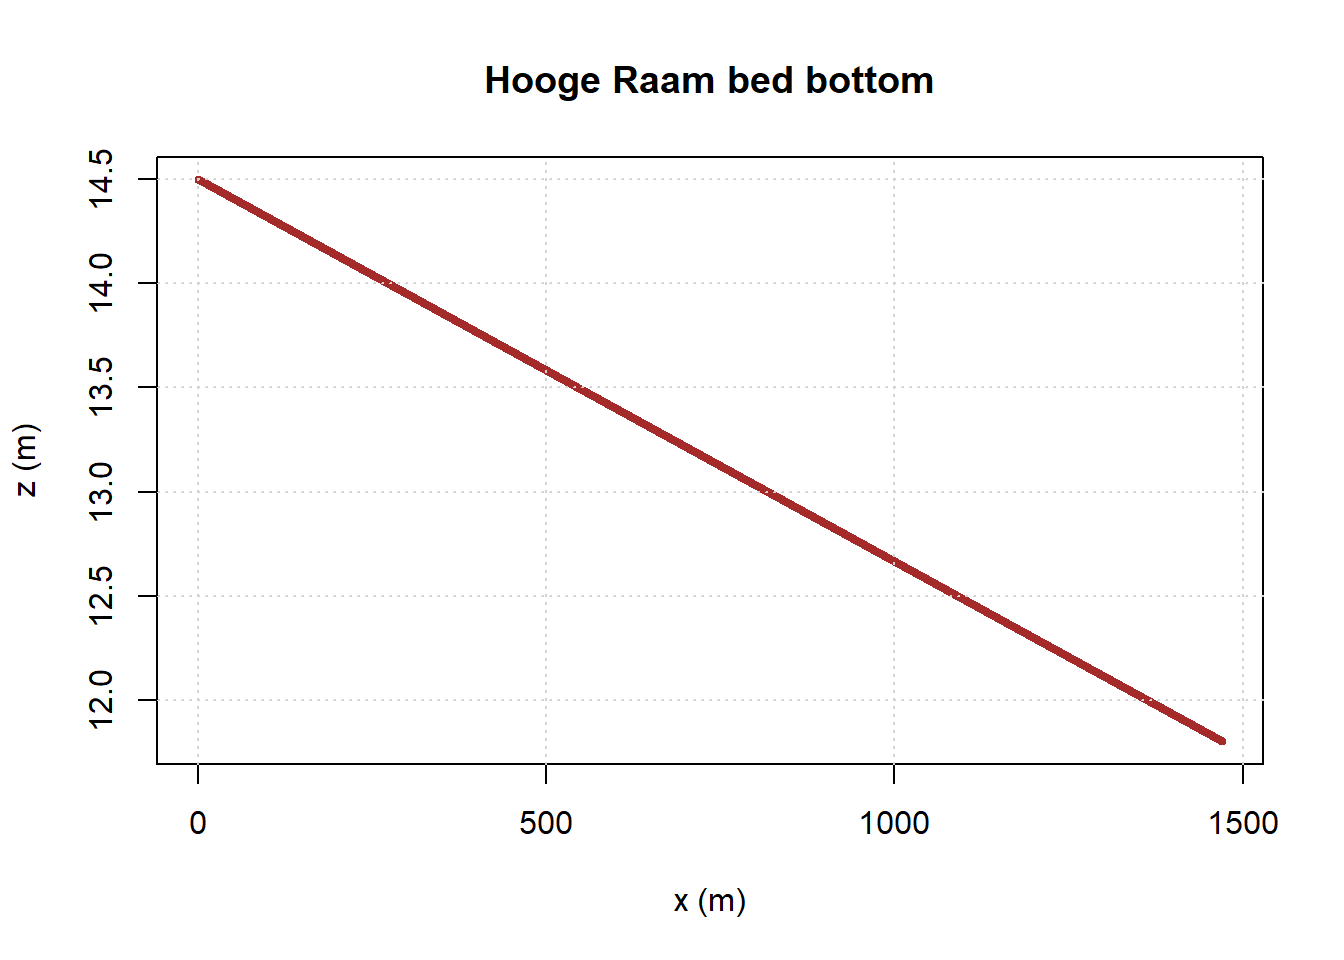
\includegraphics{start_Hooge_raam_coupling_files/figure-latex/unnamed-chunk-2-1.pdf}

This bottom slope brings the gravity into the equations: the higher this
slope, the larger the influence of the gravity on the water flow.

\hypertarget{cross-section-geometry}{%
\subsection{Cross section geometry}\label{cross-section-geometry}}

The cross section can in general have a complex and spatially varying
form. Her we take just a simple trapezoidal profile with a constant
bottom width \(b\) and constant side slope \(m\):

\begin{Shaded}
\begin{Highlighting}[]
\NormalTok{HR.b}\OtherTok{=}\FloatTok{2.1}   \CommentTok{\# bottom  width}
\NormalTok{HR.m}\OtherTok{=}\FloatTok{1.5}   \CommentTok{\# side slope}
\end{Highlighting}
\end{Shaded}

The water level with respect to the bottom of this cross section is
called the \emph{water depth} and will be denoted by \(a\). To make a
plot of the cross section we need to calculate the width for a whole
range of possible water depths.

For a trapezoidal cross section this results in:

\begin{Shaded}
\begin{Highlighting}[]
\NormalTok{HR.width }\OtherTok{=} \ControlFlowTok{function}\NormalTok{(a)}
\NormalTok{\{}
  \FunctionTok{return}\NormalTok{(HR.b}\SpecialCharTok{+}\DecValTok{2}\SpecialCharTok{*}\NormalTok{HR.m}\SpecialCharTok{*}\NormalTok{a)}
\NormalTok{\}}
\end{Highlighting}
\end{Shaded}

The next chunk creates a plot of the cross section

\begin{Shaded}
\begin{Highlighting}[]
\NormalTok{arange}\OtherTok{=}\FunctionTok{seq}\NormalTok{(}\DecValTok{0}\NormalTok{,}\FloatTok{1.5}\NormalTok{,}\AttributeTok{length=}\DecValTok{100}\NormalTok{) }\CommentTok{\# large enough of possible depth values }
\NormalTok{widthrange }\OtherTok{=} \FunctionTok{HR.width}\NormalTok{(arange)}
\FunctionTok{plot}\NormalTok{(}\FunctionTok{c}\NormalTok{(}\SpecialCharTok{{-}}\FunctionTok{rev}\NormalTok{(widthrange}\SpecialCharTok{/}\DecValTok{2}\NormalTok{),widthrange}\SpecialCharTok{/}\DecValTok{2}\NormalTok{),}\FunctionTok{c}\NormalTok{(}\FunctionTok{rev}\NormalTok{(arange),arange),}
     \AttributeTok{xlab=}\StringTok{"y"}\NormalTok{,}\AttributeTok{ylab=}\StringTok{"a"}\NormalTok{,}\AttributeTok{main=}\StringTok{"cross section"}\NormalTok{,}\AttributeTok{type=}\StringTok{"l"}\NormalTok{,}\AttributeTok{lwd=}\DecValTok{5}\NormalTok{,}\AttributeTok{col=}\StringTok{"brown"}\NormalTok{)}
\FunctionTok{grid}\NormalTok{(}\AttributeTok{col=}\StringTok{"black"}\NormalTok{)}
\end{Highlighting}
\end{Shaded}

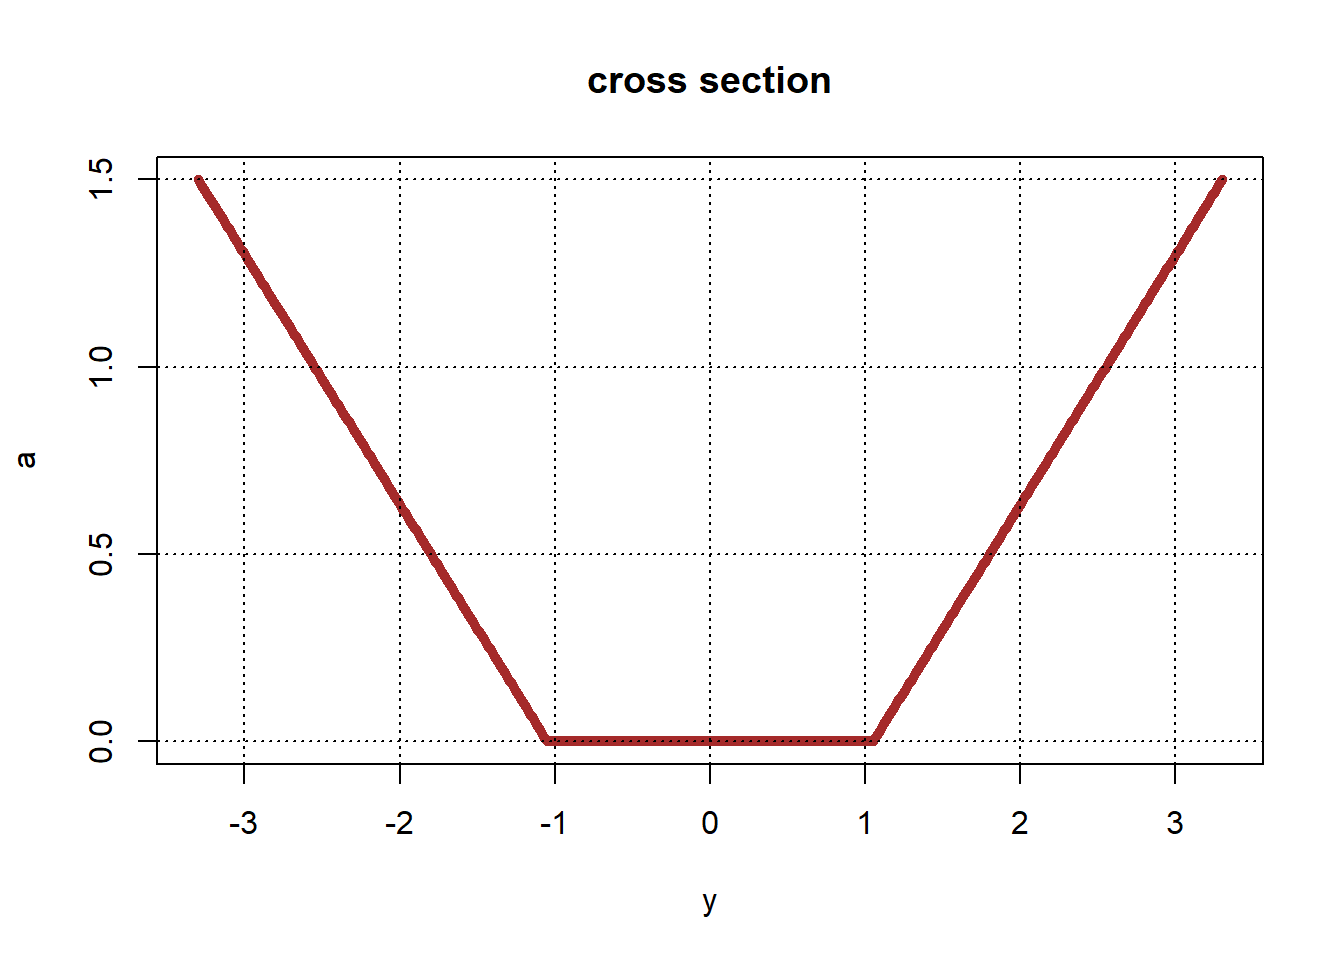
\includegraphics{start_Hooge_raam_coupling_files/figure-latex/unnamed-chunk-5-1.pdf}

\hypertarget{wetted-area}{%
\subsection{Wetted area}\label{wetted-area}}

One of the important cross section functions is the wetted area. It was
in the St-Venant equation denoted by \(A\). For a trapezoidal cross
section this can be easily calculated by the following function:

\begin{Shaded}
\begin{Highlighting}[]
\NormalTok{HR.A }\OtherTok{=} \ControlFlowTok{function}\NormalTok{(a)}
\NormalTok{\{}
  \FunctionTok{return}\NormalTok{(HR.b}\SpecialCharTok{*}\NormalTok{a}\SpecialCharTok{+}\NormalTok{HR.m}\SpecialCharTok{*}\NormalTok{a}\SpecialCharTok{\^{}}\DecValTok{2}\NormalTok{)}
\NormalTok{\}}
\end{Highlighting}
\end{Shaded}

One of the reasons that this wetted cross section is so important is
because of the important formula \(Q = v A\), were \(Q\) is the
discharge, \(v\) is the velocity and \(A\) is the wetted cross section.
Some typical (max) velocities depending of the soil type are given the
table below

\begin{longtable}[]{@{}cc@{}}
\caption{source: Cultuurtechnisch Vademecum 1988}\tabularnewline
\toprule\noalign{}
Soil type & velocity m/s \\
\midrule\noalign{}
\endfirsthead
\toprule\noalign{}
Soil type & velocity m/s \\
\midrule\noalign{}
\endhead
\bottomrule\noalign{}
\endlastfoot
clay/loam/loess & 0.60 - 0.80 \\
sand/solid peat & 0.30 - 0.60 \\
coarse sand & 0.20 - 0.50 \\
fine sand/soft peat & 0.15 - 0.30 \\
\end{longtable}

As can be seen in the function above that the wetted cross section is
dependent on the water depth \(a\). One way to see the influence of the
wetted cross section on the discharge is to investigate the relationship
between \(Q\) and \(a\) for fixed velocities. Here is a typical example
(it is customary to plot water depths on the vertical axis):

\begin{Shaded}
\begin{Highlighting}[]
\NormalTok{Arange }\OtherTok{=}  \FunctionTok{HR.A}\NormalTok{(arange)}
\NormalTok{vel }\OtherTok{=} \FloatTok{0.50} \CommentTok{\#m/s velocity for coarse sand}
\NormalTok{Qrange }\OtherTok{=}\NormalTok{ vel}\SpecialCharTok{*}\NormalTok{Arange}
\FunctionTok{plot}\NormalTok{(Qrange,arange,}
     \AttributeTok{main=}\StringTok{"Hooge Raam Q{-}a relation for fixed velocity v"}\NormalTok{,}
     \AttributeTok{xlab=}\StringTok{"Q (m\^{}3/s)"}\NormalTok{,}\AttributeTok{ylab=}\StringTok{"a (m)"}\NormalTok{,}\AttributeTok{col=}\StringTok{"brown"}\NormalTok{,}\AttributeTok{lwd=}\DecValTok{3}\NormalTok{,}\AttributeTok{type=}\StringTok{"l"}\NormalTok{)}
\FunctionTok{legend}\NormalTok{(}\StringTok{"bottomright"}\NormalTok{, }\AttributeTok{inset=}\NormalTok{.}\DecValTok{05}\NormalTok{, }\AttributeTok{title=}\StringTok{"v (m/s)"}\NormalTok{,}
       \FunctionTok{c}\NormalTok{(}\StringTok{"0.5"}\NormalTok{), }\AttributeTok{col=}\FunctionTok{c}\NormalTok{(}\StringTok{"brown"}\NormalTok{),}\AttributeTok{lwd=}\DecValTok{3}\NormalTok{,}\AttributeTok{horiz=}\ConstantTok{TRUE}\NormalTok{)}
\FunctionTok{grid}\NormalTok{(}\AttributeTok{col=}\StringTok{"black"}\NormalTok{)}
\end{Highlighting}
\end{Shaded}

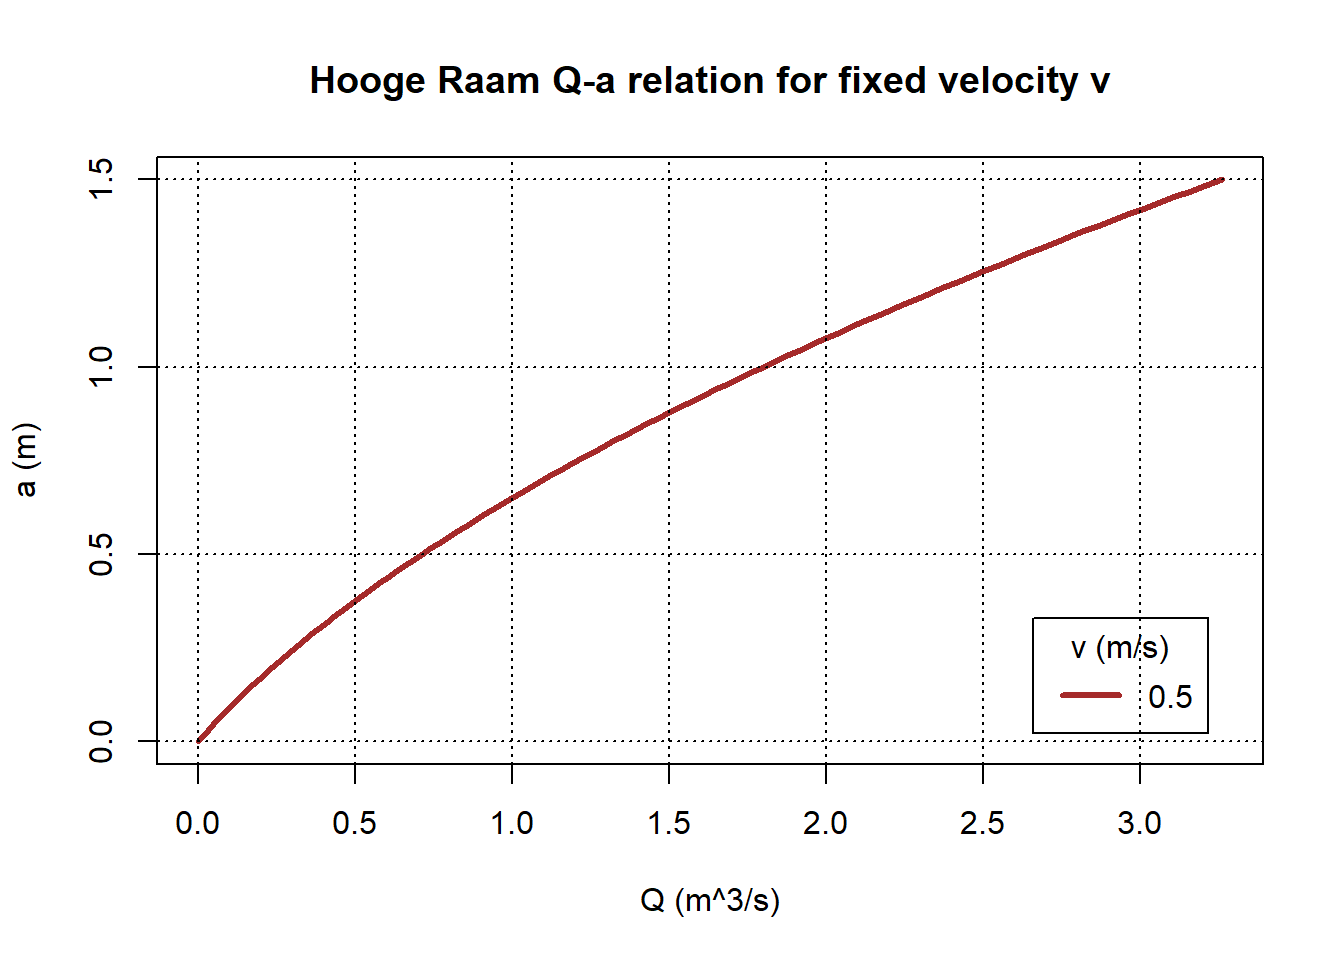
\includegraphics{start_Hooge_raam_coupling_files/figure-latex/unnamed-chunk-7-1.pdf}

Velocities higher than 1 m/s are however rather atypical.

Fill the chunk below (replace all XXX) with a code that combines in
one\\
plot the a-Q for four realistic velocities.

\begin{Shaded}
\begin{Highlighting}[]
\NormalTok{Arange }\OtherTok{=}  \FunctionTok{HR.A}\NormalTok{(arange) }\CommentTok{\#Calculating wetted area}
\NormalTok{Q1range }\OtherTok{=} \FloatTok{0.15}\SpecialCharTok{*}\NormalTok{Arange  }\CommentTok{\#Clay/loam/loess velocity}
\NormalTok{Q2range}\OtherTok{=}  \FloatTok{0.20}\SpecialCharTok{*}\NormalTok{Arange   }\CommentTok{\#Sand/solid peat velocity}
\NormalTok{Q3range}\OtherTok{=}  \FloatTok{0.30}\SpecialCharTok{*}\NormalTok{Arange  }\CommentTok{\#Coarse sand }
\NormalTok{Q4range }\OtherTok{=} \FloatTok{0.60}\SpecialCharTok{*}\NormalTok{Arange     }\CommentTok{\#Fine sand/soft peat}
\FunctionTok{plot}\NormalTok{(Q4range,arange,   }\CommentTok{\#Make a plot of fine sand}
     \AttributeTok{main=}\StringTok{"Hooge Raam Q{-}a relation for fixed velocity v"}\NormalTok{, }\CommentTok{\#{-}{-}}
     \AttributeTok{xlab=}\StringTok{"Q (m\^{}3/s)"}\NormalTok{,}\AttributeTok{ylab=}\StringTok{"a (m)"}\NormalTok{,}\AttributeTok{col=}\StringTok{"brown"}\NormalTok{,}\AttributeTok{lwd=}\DecValTok{3}\NormalTok{,}\AttributeTok{type=}\StringTok{"l"}\NormalTok{, }\AttributeTok{ylim=}\FunctionTok{c}\NormalTok{(}\DecValTok{0}\NormalTok{,}\DecValTok{2}\NormalTok{), }\AttributeTok{xlim =} \FunctionTok{c}\NormalTok{(}\DecValTok{0}\NormalTok{,}\DecValTok{2}\NormalTok{)) }\CommentTok{\#{-}{-}}
\FunctionTok{lines}\NormalTok{(Q3range,arange,}\AttributeTok{lwd=}\DecValTok{3}\NormalTok{,}\AttributeTok{col=}\StringTok{"blue"}\NormalTok{) }\CommentTok{\#Adding plot of coarse sand}
\FunctionTok{lines}\NormalTok{(Q2range,arange,}\AttributeTok{lwd=}\DecValTok{3}\NormalTok{,}\AttributeTok{col=}\StringTok{"red"}\NormalTok{)  }\CommentTok{\#Adding plot of sand/solid peat}
\FunctionTok{lines}\NormalTok{(Q1range,arange,}\AttributeTok{lwd=}\DecValTok{3}\NormalTok{,}\AttributeTok{col=}\StringTok{"green"}\NormalTok{) }\CommentTok{\#Adding plot of clay/loam/loess}

\DocumentationTok{\#\# FIX LEGEND HERE}
\CommentTok{\#legend("bottomright", inset=c({-}0.2,1.0), title="v (m/s)", \#Adding the legend}
\CommentTok{\#c("clay","sand","coarse sand","fine sand"), col=c("green","red","blue","brown"),lwd=3,horiz=TRUE) \#Color the difference scenario}

\FunctionTok{grid}\NormalTok{(}\AttributeTok{col=}\StringTok{"black"}\NormalTok{) }\CommentTok{\#Making the color of the grid to be black}
\end{Highlighting}
\end{Shaded}

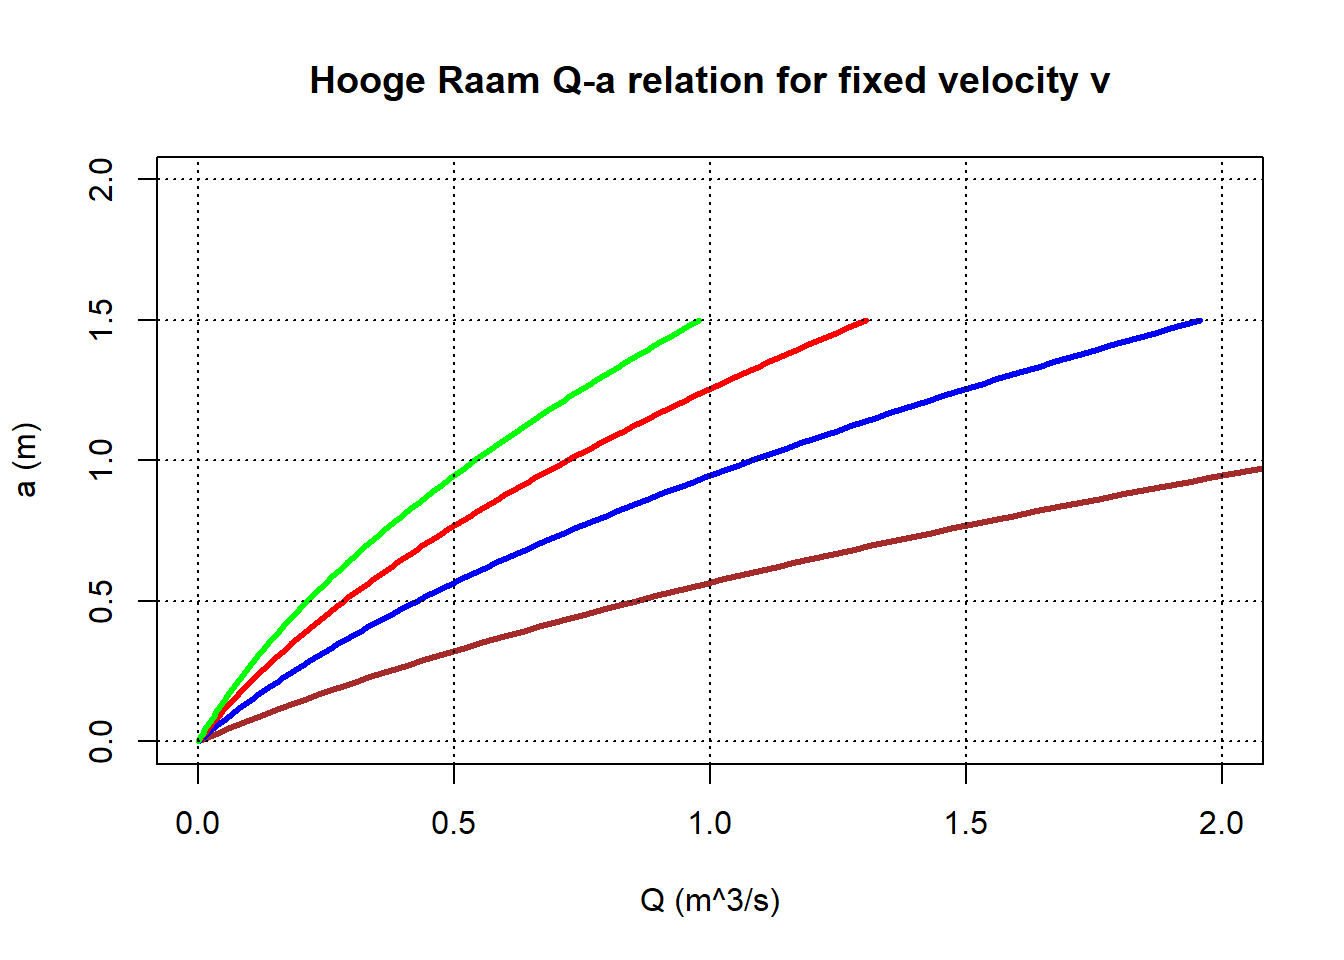
\includegraphics{start_Hooge_raam_coupling_files/figure-latex/unnamed-chunk-8-1.pdf}

\hypertarget{equilibrium-discharge}{%
\subsection{Equilibrium discharge}\label{equilibrium-discharge}}

But of course usually both and \(A\) and \(v\) change if the water depth
\(a\) changes.

For equilibrium situations this relationship can be investigated through
formulas. Equilibrium means that the water depth is constant in space
(\(\frac{\partial a}{\partial x} = 0\)) in terms of the St-Venant
equations of the introduction) and time. For this situation the open
water equation simplifies into;
\[S_0 = S_f = \frac{n^2\; Q^2}{A^2\; R^{4/3}}\]

From this one can derive:
\[Q_\mathrm{equi} = \frac{\sqrt{S_o}}{n} A\; R^{2/3}\] where

\begin{itemize}
\item
  \(S_o\): bottom slope (as calculated above)
\item
  \(n\): Manning coefficient: the higher this number, the more friction,
  typical values are around 0.04, but difficult to assess
\item
  \(A\): the wetted cross section, as discussed and calculated above
\item
  \(R\): hydraulic radius. Formally defined as wetted Area divided by
  the wetted perimeter(\(R=\frac {A}{P}\)), as in the next chunk:
\end{itemize}

\begin{Shaded}
\begin{Highlighting}[]
\NormalTok{HR.n }\OtherTok{=} \FloatTok{0.045} 

\NormalTok{HR.R }\OtherTok{=} \ControlFlowTok{function}\NormalTok{(a)}
\NormalTok{\{}
  \FunctionTok{return}\NormalTok{((HR.b}\SpecialCharTok{*}\NormalTok{a}\SpecialCharTok{+}\NormalTok{HR.m}\SpecialCharTok{*}\NormalTok{a}\SpecialCharTok{\^{}}\DecValTok{2}\NormalTok{)}\SpecialCharTok{/}\NormalTok{(HR.b}\SpecialCharTok{+}\DecValTok{2}\SpecialCharTok{*}\FunctionTok{sqrt}\NormalTok{(}\DecValTok{1}\SpecialCharTok{+}\NormalTok{HR.m}\SpecialCharTok{\^{}}\DecValTok{2}\NormalTok{)}\SpecialCharTok{*}\NormalTok{a))}
\NormalTok{\}}
\NormalTok{HR.Qequi }\OtherTok{=} \ControlFlowTok{function}\NormalTok{(a)}
\NormalTok{\{}
\NormalTok{  R }\OtherTok{=} \FunctionTok{HR.R}\NormalTok{(a)}
\NormalTok{  A }\OtherTok{=} \FunctionTok{HR.A}\NormalTok{(a)}
\NormalTok{  Q }\OtherTok{=} \FunctionTok{sqrt}\NormalTok{(HR.So)}\SpecialCharTok{/}\NormalTok{HR.n}\SpecialCharTok{*}\NormalTok{A}\SpecialCharTok{*}\NormalTok{R}\SpecialCharTok{\^{}}\NormalTok{(}\DecValTok{2}\SpecialCharTok{/}\DecValTok{3}\NormalTok{) }\CommentTok{\#\% =}
  \FunctionTok{return}\NormalTok{(}\FunctionTok{sqrt}\NormalTok{(HR.So)}\SpecialCharTok{/}\NormalTok{HR.n}\SpecialCharTok{*}\NormalTok{A}\SpecialCharTok{*}\NormalTok{R}\SpecialCharTok{\^{}}\NormalTok{(}\DecValTok{2}\SpecialCharTok{/}\DecValTok{3}\NormalTok{))}
\NormalTok{\}}

\NormalTok{Qequirange }\OtherTok{=} \FunctionTok{HR.Qequi}\NormalTok{(arange)}
\FunctionTok{plot}\NormalTok{(Qequirange,arange,}
     \AttributeTok{main=}\StringTok{"Hooge Raam Q{-}a equilibrium"}\NormalTok{,}
     \AttributeTok{xlab=}\StringTok{"Qequi"}\NormalTok{,}\AttributeTok{ylab=}\StringTok{"a"}\NormalTok{,}\AttributeTok{lwd=}\DecValTok{3}\NormalTok{,}\AttributeTok{col=}\StringTok{"blue"}\NormalTok{,}\AttributeTok{type=}\StringTok{"l"}\NormalTok{)}
\FunctionTok{grid}\NormalTok{(}\AttributeTok{col=}\StringTok{"black"}\NormalTok{)}
\end{Highlighting}
\end{Shaded}

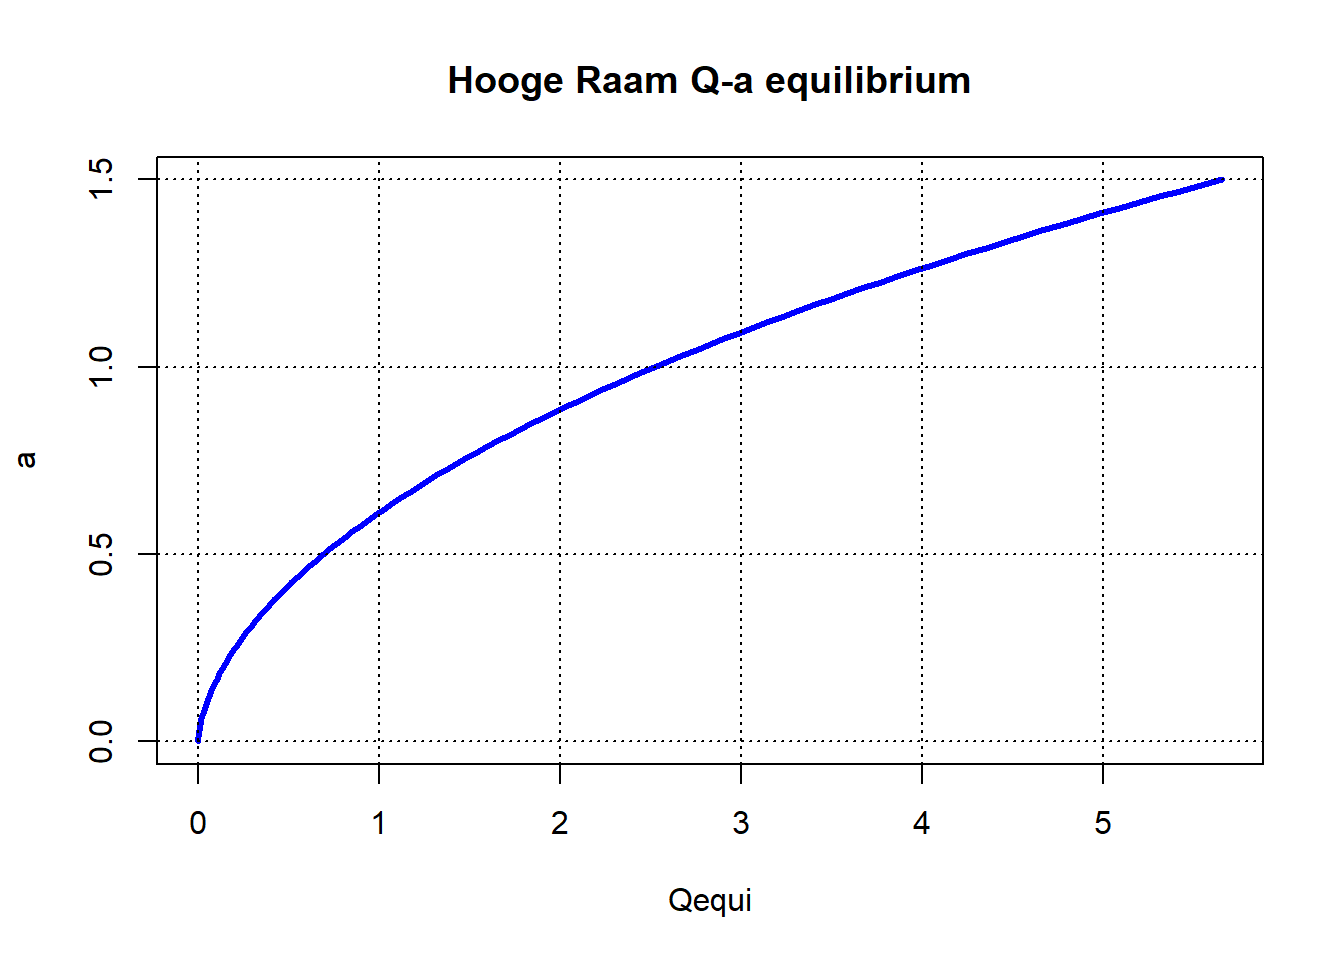
\includegraphics{start_Hooge_raam_coupling_files/figure-latex/unnamed-chunk-9-1.pdf}

Sometimes the question is posed the other way around. Assume that one
wants to drain a constant intensity of 10 \(mm/day\) of an area of the
size of 30 \(km^2\) through this river.

Step1: calculate the discharge through the river.

\begin{Shaded}
\begin{Highlighting}[]
\NormalTok{area }\OtherTok{=} \DecValTok{30} \CommentTok{\# km\^{}2}
\NormalTok{area }\OtherTok{=}\NormalTok{ area }\SpecialCharTok{*}\NormalTok{(}\DecValTok{1000}\NormalTok{)}\SpecialCharTok{\^{}}\DecValTok{2} \CommentTok{\# m\^{}2}
\NormalTok{I }\OtherTok{=} \DecValTok{10} \CommentTok{\# mm /day}
\NormalTok{I }\OtherTok{=}\NormalTok{ I}\SpecialCharTok{/}\NormalTok{(}\DecValTok{1000}\SpecialCharTok{*}\DecValTok{24}\SpecialCharTok{*}\DecValTok{3600}\NormalTok{) }\CommentTok{\# m/s \#+ = }
\NormalTok{Q }\OtherTok{=}\NormalTok{ I}\SpecialCharTok{*}\NormalTok{area}
\end{Highlighting}
\end{Shaded}

Now we want to calculate the water level corresponding to the
equilibrium discharge just calculated. We can use the plot made above,
or we can use the following chunk to find the water level corresponding
to the calculated discharge rate.

\begin{Shaded}
\begin{Highlighting}[]
\FunctionTok{library}\NormalTok{(nleqslv)}
\end{Highlighting}
\end{Shaded}

\begin{verbatim}
## Warning: package 'nleqslv' was built under R version 4.3.2
\end{verbatim}

\begin{Shaded}
\begin{Highlighting}[]
\NormalTok{tosolve }\OtherTok{=} \ControlFlowTok{function}\NormalTok{(a)\{}\FunctionTok{return}\NormalTok{ (}\FunctionTok{HR.Qequi}\NormalTok{(a)}\SpecialCharTok{{-}}\NormalTok{Q)\}}
\NormalTok{aequi }\OtherTok{=} \FunctionTok{nleqslv}\NormalTok{(}\DecValTok{1}\NormalTok{,tosolve)}\SpecialCharTok{$}\NormalTok{x}
\FunctionTok{print}\NormalTok{(aequi)}
\end{Highlighting}
\end{Shaded}

\begin{verbatim}
## [1] 1.177077
\end{verbatim}

Repeat the calculation above for the rainfall intensities between 0.5
mm/day and 15 mm/day and make a plot of the water depths vs these
intensities.

\begin{Shaded}
\begin{Highlighting}[]
\NormalTok{Is }\OtherTok{=} \FunctionTok{seq}\NormalTok{(}\FloatTok{0.5}\NormalTok{,}\DecValTok{15}\NormalTok{,}\AttributeTok{length=}\DecValTok{100}\NormalTok{)}
\NormalTok{aequis }\OtherTok{=} \FunctionTok{c}\NormalTok{()}
\ControlFlowTok{for}\NormalTok{( i }\ControlFlowTok{in} \DecValTok{1}\SpecialCharTok{:}\FunctionTok{length}\NormalTok{(Is))}
\NormalTok{\{}
\NormalTok{  I }\OtherTok{=}\NormalTok{ Is[i]}\SpecialCharTok{/}\NormalTok{(}\DecValTok{3600}\SpecialCharTok{*}\DecValTok{24}\SpecialCharTok{*}\DecValTok{1000}\NormalTok{)}
\NormalTok{  Q }\OtherTok{=}\NormalTok{ I}\SpecialCharTok{*}\NormalTok{area                }
\NormalTok{  tosolve }\OtherTok{=} \ControlFlowTok{function}\NormalTok{(a)\{}\FunctionTok{return}\NormalTok{ (}\FunctionTok{HR.Qequi}\NormalTok{(a)}\SpecialCharTok{{-}}\NormalTok{Q)\}}
\NormalTok{  aequis[i] }\OtherTok{=} \FunctionTok{nleqslv}\NormalTok{(}\DecValTok{1}\NormalTok{,tosolve)}\SpecialCharTok{$}\NormalTok{x}
\NormalTok{\}}
\FunctionTok{plot}\NormalTok{(Is,aequis,}\AttributeTok{type=}\StringTok{"l"}\NormalTok{,}\AttributeTok{col=}\StringTok{"blue"}\NormalTok{,}\AttributeTok{lwd=}\DecValTok{3}\NormalTok{, }\AttributeTok{main=}\StringTok{"Water Depth for Different Rain Intensities"}\NormalTok{, }\AttributeTok{xlab =} \StringTok{"Rainfall intensity (mm/day)"}\NormalTok{, }\AttributeTok{ylab =} \StringTok{"Steady state water level (m)"}\NormalTok{)}
\FunctionTok{grid}\NormalTok{(}\AttributeTok{col=}\StringTok{"black"}\NormalTok{)}
\end{Highlighting}
\end{Shaded}

\hypertarget{the-downstream-weir}{%
\section{The downstream weir}\label{the-downstream-weir}}

\hypertarget{geometry-of-the-weir}{%
\subsection{Geometry of the weir}\label{geometry-of-the-weir}}

See the following graph

\begin{Shaded}
\begin{Highlighting}[]
\NormalTok{HR.weir.width }\OtherTok{=} \FloatTok{2.25}  \CommentTok{\#m width of the weir floor }
\NormalTok{HR.weir.crest }\OtherTok{=} \DecValTok{1} \CommentTok{\#m above bottom river}
\CommentTok{\# draw weir in cross section}
\FunctionTok{plot}\NormalTok{(}\FunctionTok{c}\NormalTok{(}\SpecialCharTok{{-}}\FunctionTok{rev}\NormalTok{(widthrange}\SpecialCharTok{/}\DecValTok{2}\NormalTok{),widthrange}\SpecialCharTok{/}\DecValTok{2}\NormalTok{),}\FunctionTok{c}\NormalTok{(}\FunctionTok{rev}\NormalTok{(arange),arange),}
     \AttributeTok{xlab=}\StringTok{"y"}\NormalTok{,}\AttributeTok{ylab=}\StringTok{"a"}\NormalTok{,}\AttributeTok{main=}\StringTok{"cross section"}\NormalTok{,}\AttributeTok{type=}\StringTok{"l"}\NormalTok{,}\AttributeTok{lwd=}\DecValTok{5}\NormalTok{,}\AttributeTok{col=}\StringTok{"brown"}\NormalTok{)}
\FunctionTok{lines}\NormalTok{(}\FunctionTok{c}\NormalTok{(}\SpecialCharTok{{-}}\NormalTok{HR.weir.width}\SpecialCharTok{/}\DecValTok{2}\NormalTok{,}\SpecialCharTok{{-}}\NormalTok{HR.weir.width}\SpecialCharTok{/}\DecValTok{2}\NormalTok{,HR.weir.width}\SpecialCharTok{/}\DecValTok{2}\NormalTok{,HR.weir.width}\SpecialCharTok{/}\DecValTok{2}\NormalTok{),}
      \FunctionTok{c}\NormalTok{(}\FunctionTok{max}\NormalTok{(arange),HR.weir.crest,HR.weir.crest,}\FunctionTok{max}\NormalTok{(arange))}
\NormalTok{      ,}\AttributeTok{col=}\StringTok{"blue"}\NormalTok{,}\AttributeTok{lwd=}\DecValTok{3}\NormalTok{)}
\FunctionTok{legend}\NormalTok{(}\StringTok{"bottomright"}\NormalTok{, }\AttributeTok{inset=}\NormalTok{.}\DecValTok{05}\NormalTok{,}
       \FunctionTok{c}\NormalTok{(}\StringTok{"river"}\NormalTok{,}\StringTok{"weir"}\NormalTok{), }\AttributeTok{col=}\FunctionTok{c}\NormalTok{(}\StringTok{"brown"}\NormalTok{,}\StringTok{"blue"}\NormalTok{),}\AttributeTok{lwd=}\DecValTok{3}\NormalTok{,}\AttributeTok{horiz=}\ConstantTok{FALSE}\NormalTok{)}
\FunctionTok{grid}\NormalTok{(}\AttributeTok{col=}\StringTok{"black"}\NormalTok{)}
\end{Highlighting}
\end{Shaded}

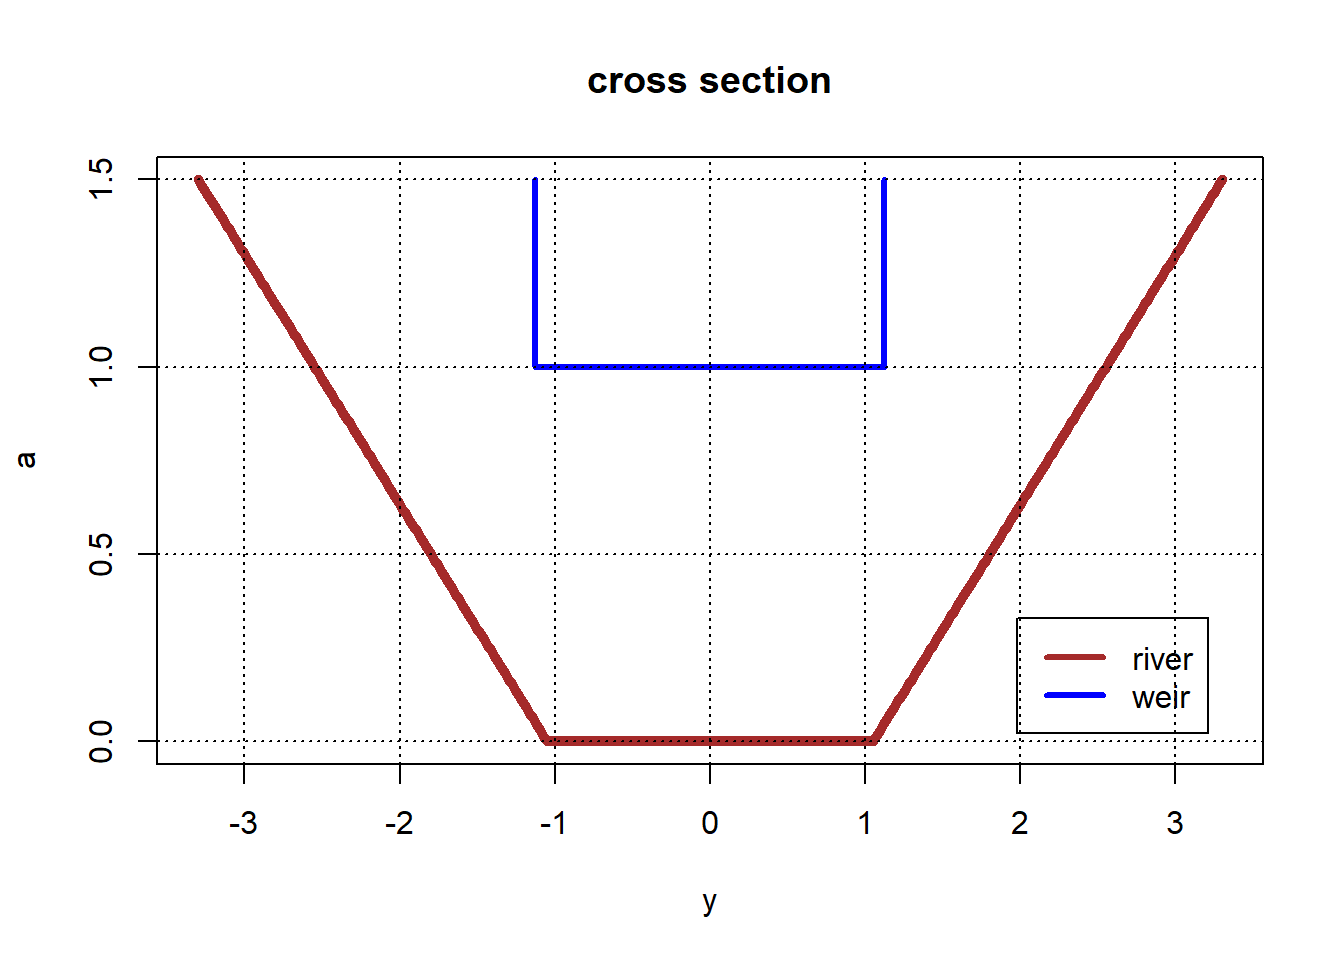
\includegraphics{start_Hooge_raam_coupling_files/figure-latex/unnamed-chunk-13-1.pdf}

\hypertarget{weir-q-a-relation}{%
\subsection{Weir Q-a relation}\label{weir-q-a-relation}}

The amount of water flowing over a weir is a function of the water
height above the crest. For a rectangular weir this is a well known
formula:
\[Q_\mathrm{weir} = 1.83\; B_\mathrm{weir}\; (a-c_\mathrm{weir})^{3/2}\]

Finish the code below such that the function calculates discharges
according to the formula above.

\begin{Shaded}
\begin{Highlighting}[]
\NormalTok{HR.weirQ }\OtherTok{=} \ControlFlowTok{function}\NormalTok{(a)}
\NormalTok{\{}
\NormalTok{  a[a}\SpecialCharTok{\textless{}}\NormalTok{HR.weir.crest] }\OtherTok{=}\NormalTok{ HR.weir.crest}
  \FunctionTok{return}\NormalTok{(XXXX)}
\NormalTok{\}}

\NormalTok{weirQrange }\OtherTok{=} \FunctionTok{HR.weirQ}\NormalTok{(arange)}

\FunctionTok{plot}\NormalTok{(Qequirange,arange,}\AttributeTok{main=}\StringTok{"Qequi and Qweir for HoogeRaam"}\NormalTok{,}
     \AttributeTok{xlab=}\StringTok{"Qequi"}\NormalTok{,}\AttributeTok{ylab=}\StringTok{"a"}\NormalTok{,}\AttributeTok{lwd=}\DecValTok{3}\NormalTok{,}\AttributeTok{col=}\StringTok{"blue"}\NormalTok{,}\AttributeTok{type=}\StringTok{"l"}\NormalTok{)}
\FunctionTok{lines}\NormalTok{(weirQrange,arange,}\AttributeTok{lwd=}\DecValTok{3}\NormalTok{,}\AttributeTok{col=}\StringTok{"red"}\NormalTok{)}
\FunctionTok{legend}\NormalTok{(}\StringTok{"bottomright"}\NormalTok{, }\AttributeTok{inset=}\NormalTok{.}\DecValTok{05}\NormalTok{,}
       \FunctionTok{c}\NormalTok{(}\StringTok{"Qequiriver"}\NormalTok{,}\StringTok{"Qweir"}\NormalTok{), }\AttributeTok{col=}\FunctionTok{c}\NormalTok{(}\StringTok{"blue"}\NormalTok{,}\StringTok{"red"}\NormalTok{),}\AttributeTok{lwd=}\DecValTok{3}\NormalTok{,}\AttributeTok{horiz=}\ConstantTok{FALSE}\NormalTok{)}
\FunctionTok{grid}\NormalTok{(}\AttributeTok{col=}\StringTok{"black"}\NormalTok{)}
\end{Highlighting}
\end{Shaded}

\hypertarget{rough-backwater-approximation}{%
\section{Rough backwater
approximation}\label{rough-backwater-approximation}}

For any given fixed discharge \(Q\) that goes through the Hooge Raam, we
can calculate two water levels with the information above:

\begin{itemize}
\item
  a water depth and level at the weir
\item
  an equilibrium water depth and level far upstream of the weir
\end{itemize}

In between the water levels will vary between these two. Here we first
are going to calculate these levels and then just as a first rough
approximation interpolate linear in between.

Calculate for Q=1.2 the water depth at the weir and the water depth at
the upstream end

\begin{Shaded}
\begin{Highlighting}[]
\FunctionTok{library}\NormalTok{(nleqslv)}
\NormalTok{Q }\OtherTok{=} \FloatTok{1.2}
\NormalTok{tosolve }\OtherTok{=} \ControlFlowTok{function}\NormalTok{(a)\{}\FunctionTok{return}\NormalTok{ (XXXX}\SpecialCharTok{{-}}\NormalTok{Q)\}}
\NormalTok{aequi }\OtherTok{=} \FunctionTok{nleqslv}\NormalTok{(}\DecValTok{1}\NormalTok{,tosolve)}\SpecialCharTok{$}\NormalTok{x}
\FunctionTok{print}\NormalTok{(aequi)}
\NormalTok{tosolve }\OtherTok{=} \ControlFlowTok{function}\NormalTok{(a)\{}\FunctionTok{return}\NormalTok{ (XXXX}\SpecialCharTok{{-}}\NormalTok{Q)\}}
\NormalTok{aweir }\OtherTok{=} \FunctionTok{nleqslv}\NormalTok{(}\FloatTok{1.1}\NormalTok{,tosolve)}\SpecialCharTok{$}\NormalTok{x}
\FunctionTok{print}\NormalTok{(aweir)}
\end{Highlighting}
\end{Shaded}

Make a function for the rough linear approximation and plot it

\begin{Shaded}
\begin{Highlighting}[]
\NormalTok{HR.bwrough }\OtherTok{=} \FunctionTok{approxfun}\NormalTok{(HR.domain,}
                       \FunctionTok{c}\NormalTok{(HR.botelev.upstream}\SpecialCharTok{+}\NormalTok{XXXX,HR.botelev.dnstream}\SpecialCharTok{+}\NormalTok{XXXX),}\AttributeTok{rule=}\DecValTok{2}\NormalTok{) }\CommentTok{\#\% aequi \#\% aweir}
\FunctionTok{plot}\NormalTok{(HR.domain,}\FunctionTok{HR.bwrough}\NormalTok{(HR.domain),}\AttributeTok{ylim=}\FunctionTok{c}\NormalTok{(HR.botelev.dnstream,HR.botelev.upstream}\SpecialCharTok{+}\NormalTok{aequi),}
     \AttributeTok{main=}\FunctionTok{paste}\NormalTok{(}\StringTok{"rough level approx for Q="}\NormalTok{,Q),}
     \AttributeTok{xlab=}\StringTok{"l (m)"}\NormalTok{,}\AttributeTok{ylab=}\StringTok{"h (m)"}\NormalTok{,}\AttributeTok{col=}\StringTok{"blue"}\NormalTok{,}\AttributeTok{lwd=}\DecValTok{4}\NormalTok{,}\AttributeTok{type=}\StringTok{"l"}\NormalTok{)}
\FunctionTok{lines}\NormalTok{(HR.domain,}\FunctionTok{HR.zb}\NormalTok{(HR.domain),}\AttributeTok{col=}\StringTok{"brown"}\NormalTok{,}\AttributeTok{lwd=}\DecValTok{4}\NormalTok{)}
\end{Highlighting}
\end{Shaded}

\hypertarget{setup-of-base-backwater-model}{%
\section{Setup of base backwater
model}\label{setup-of-base-backwater-model}}

The previous backwater approximation is too rough. In reality the water
levels will vary non-linear (but still very smoothly). A 1D flow model
has to be setup to calculate these levels. So the 1D flow library needs
to be loaded:

\begin{Shaded}
\begin{Highlighting}[]
\FunctionTok{library}\NormalTok{(FVFE1D)}
\end{Highlighting}
\end{Shaded}

\begin{verbatim}
## Loading required package: Matrix
\end{verbatim}

\hypertarget{the-choice-of-state}{%
\subsection{The choice of state}\label{the-choice-of-state}}

For all kind of local calculations the water depth \(a\) is the most
common choice. For non-local problems as the calculation of a backwater
curve, the \emph{water level} with respect to AMSL (the \(h\) in the
plot above) is the most common choice. These two quantities are
connected through the river, bottom height:\\
\[
  h = z_b(x)+a 
\]

For the Hooge Raam, a function for the bottom was already given:
\textbf{HR.zb} (see above).

\hypertarget{the-equation}{%
\subsection{The equation}\label{the-equation}}

Finish the function definition below:

\begin{Shaded}
\begin{Highlighting}[]
\NormalTok{HR.a }\OtherTok{=} \ControlFlowTok{function}\NormalTok{(x,XXXX)}
\NormalTok{\{}
  \FunctionTok{return}\NormalTok{(XXXX}\SpecialCharTok{{-}}\FunctionTok{HR.zb}\NormalTok{(x)) }\CommentTok{\#}
\NormalTok{\}}
\end{Highlighting}
\end{Shaded}

\hypertarget{the-internal-flux-function}{%
\subsection{The internal flux
function}\label{the-internal-flux-function}}

\hypertarget{the-theory}{%
\subsubsection{The theory}\label{the-theory}}

The most important step in defining a flow model is the definition of
the internal flux. The definition follows from the equation as given at
the start of this document:

\[
0 =  S_o - S_f - \frac{\partial a}{\partial x} 
\]

The formula for the friction slope, \(S_f\), requires now a bit more
sophistication.

The flow can now be to the right (\(Q>0\)) or to the left (\(Q<0\)).
Although in the given situation and with the current choice of domain,
the flow should be to the right and thus positive, it can not be
excluded that during the numerical calculations it may be (locally)
different. The friction slope is technically defined as the amount of
energy loss if going in the positive x-direction.

\begin{itemize}
\tightlist
\item
  if the flow is in the positive x-direction (\(Q>0\)), their should be
  loss in the positive x-direction, so the friction slope should be
  positive
\item
  if the flow is in the negative x-direction (\(Q<0\)), their should be
  loss in the negative x-direction, so the friction slope should be
  negative
\end{itemize}

These two cases can be combined into one formula:

\[
S_f = \mathrm{sign}(Q) \frac{n^2\; Q^2}{A^2\; R^{4/3}} 
\]

where the sign function is defined as in the R-language.

Use the help of R to give a definition of the sign function below:

Using this result, the simplified St-Venant can be written as:

\[
 \mathrm{sign}(Q) \; 
 \frac{n^2\; Q^2}{A^2\; R^{4/3}} = S_f = S_o - \frac{\partial a}{\partial x}  = 
 -\frac{\partial z_b}{\partial x} - \frac{\partial a}{\partial x} = 
 -\frac{\partial h}{\partial x}
\]

Rewriting this gives:
\[Q  = -\frac{1}{n}\; \mathrm{sign}\Big(\frac{\partial h}{\partial x}\Big)\; \sqrt{ \Big| \frac{\partial h}{\partial x} \Big|}\; A\; R^{2/3}\]

As you can see, the choice of \(h\) as state is convenient here.

\hypertarget{the-code}{%
\subsubsection{The code}\label{the-code}}

\begin{Shaded}
\begin{Highlighting}[]
\NormalTok{HR.Q}\OtherTok{=} \ControlFlowTok{function}\NormalTok{(x,state,gradstate)}
\NormalTok{\{}
\NormalTok{  a }\OtherTok{=} \FunctionTok{HR.a}\NormalTok{(x,state)}
\NormalTok{  R }\OtherTok{=} \FunctionTok{HR.R}\NormalTok{(a)}
\NormalTok{  A }\OtherTok{=} \FunctionTok{HR.A}\NormalTok{(a)}
  \FunctionTok{return}\NormalTok{(}\SpecialCharTok{{-}}\DecValTok{1}\SpecialCharTok{/}\NormalTok{HR.n}\SpecialCharTok{*}\FunctionTok{sign}\NormalTok{(gradstate)}\SpecialCharTok{*}\FunctionTok{sqrt}\NormalTok{(}\FunctionTok{abs}\NormalTok{(gradstate))}\SpecialCharTok{*}\NormalTok{A}\SpecialCharTok{*}\NormalTok{R}\SpecialCharTok{\^{}}\NormalTok{(}\DecValTok{2}\SpecialCharTok{/}\DecValTok{3}\NormalTok{)) }\CommentTok{\#+ (}
\NormalTok{\}}
\end{Highlighting}
\end{Shaded}

\hypertarget{model-1-the-hooge-raam-base-model}{%
\subsection{Model 1: the Hooge Raam base
model}\label{model-1-the-hooge-raam-base-model}}

\begin{Shaded}
\begin{Highlighting}[]
\NormalTok{HR.backwatermodel }\OtherTok{=} \FunctionTok{newFLOW1D}\NormalTok{(}\AttributeTok{domain=}\NormalTok{HR.domain,}\AttributeTok{systemfluxfunction =}\NormalTok{ HR.Q,}
                              \AttributeTok{name =} \StringTok{\textquotesingle{}Hooge Raam backwater\textquotesingle{}}\NormalTok{)}

\NormalTok{HR.weir.BC }\OtherTok{=} \ControlFlowTok{function}\NormalTok{(state)}
\NormalTok{\{}
  \FunctionTok{return}\NormalTok{(}\SpecialCharTok{{-}}\FunctionTok{HR.weirQ}\NormalTok{(}\FunctionTok{HR.a}\NormalTok{(HR.length,state)))}
\NormalTok{\}}
\NormalTok{HR.Qin }\OtherTok{=} \FloatTok{1.2}
\FunctionTok{set.BC.fluxstate}\NormalTok{(HR.backwatermodel,}\StringTok{"right"}\NormalTok{,HR.weir.BC)}
\FunctionTok{set.BC.fixedflux}\NormalTok{(HR.backwatermodel,}\AttributeTok{where=}\StringTok{"left"}\NormalTok{,}\StringTok{"HR.Qin"}\NormalTok{)}
\FunctionTok{set.discretisation}\NormalTok{(HR.backwatermodel,}\AttributeTok{nodes=}\FunctionTok{seq}\NormalTok{(}\DecValTok{0}\NormalTok{,HR.length,}\AttributeTok{length=}\DecValTok{50}\NormalTok{),}\AttributeTok{method=}\StringTok{\textquotesingle{}FE\textquotesingle{}}\NormalTok{)}

\FunctionTok{do.initialize}\NormalTok{(HR.backwatermodel,HR.bwrough)}

\NormalTok{HR.abovebottom }\OtherTok{=} \ControlFlowTok{function}\NormalTok{(x,state)}
\NormalTok{\{}
  \FunctionTok{return}\NormalTok{(}\FunctionTok{HR.a}\NormalTok{(x,state)}\SpecialCharTok{\textgreater{}}\FloatTok{0.1}\NormalTok{)}
\NormalTok{\}}

\FunctionTok{set.isacceptable}\NormalTok{(HR.backwatermodel,HR.abovebottom)}
\end{Highlighting}
\end{Shaded}

Discuss:

\begin{itemize}
\tightlist
\item
  The minus sign in the definition of the lower boundary condition:
\end{itemize}

\begin{itemize}
\tightlist
\item
  use the help of FVFE1D to discuss the role of the double quotes around
  HR.Qin in the definition of the upstream boundary condition:
\end{itemize}

\begin{itemize}
\tightlist
\item
  describe the acceptability condition of the model for the level in
  words:
\end{itemize}

\begin{Shaded}
\begin{Highlighting}[]
\FunctionTok{solve.steps}\NormalTok{(HR.backwatermodel)}
\FunctionTok{plot}\NormalTok{(HR.backwatermodel,}\AttributeTok{fluxplot=}\ConstantTok{TRUE}\NormalTok{)}
\end{Highlighting}
\end{Shaded}

And a nice plot to compare the rough (linear) approximation with the
smooth one:

\begin{Shaded}
\begin{Highlighting}[]
\FunctionTok{plot}\NormalTok{(HR.domain,}\FunctionTok{HR.bwrough}\NormalTok{(HR.domain),}\AttributeTok{ylim=}\FunctionTok{c}\NormalTok{(HR.botelev.downstream,HR.botelev.upstream}\SpecialCharTok{+}\NormalTok{aequi),}
     \AttributeTok{main=}\FunctionTok{paste}\NormalTok{(}\StringTok{"Backwater curve for Q="}\NormalTok{,HR.Qin),}
     \AttributeTok{xlab=}\StringTok{"l (m)"}\NormalTok{,}\AttributeTok{ylab=}\StringTok{"h (m)"}\NormalTok{,}\AttributeTok{col=}\StringTok{"green"}\NormalTok{,}\AttributeTok{lty=}\DecValTok{2}\NormalTok{,}\AttributeTok{lwd=}\DecValTok{4}\NormalTok{,}\AttributeTok{type=}\StringTok{"l"}\NormalTok{)}
\FunctionTok{lines}\NormalTok{(HR.domain,}\FunctionTok{HR.zb}\NormalTok{(HR.domain),}\AttributeTok{col=}\StringTok{"brown"}\NormalTok{,}\AttributeTok{lwd=}\DecValTok{4}\NormalTok{)}
\NormalTok{HR.states}\FloatTok{.1} \OtherTok{=} \FunctionTok{dataframe.states}\NormalTok{(HR.backwatermodel)}
\FunctionTok{lines}\NormalTok{(HR.states}\FloatTok{.1}\NormalTok{,}\AttributeTok{col=}\StringTok{"blue"}\NormalTok{,}\AttributeTok{lwd=}\DecValTok{4}\NormalTok{)}
\FunctionTok{legend}\NormalTok{(}\StringTok{"bottomleft"}\NormalTok{, }\AttributeTok{inset=}\NormalTok{.}\DecValTok{05}\NormalTok{,}
       \FunctionTok{c}\NormalTok{(}\StringTok{"bottom"}\NormalTok{,}\StringTok{"raw backwater"}\NormalTok{,}\StringTok{"true backwater"}\NormalTok{), }
       \AttributeTok{col=}\FunctionTok{c}\NormalTok{(}\StringTok{"brown"}\NormalTok{,}\StringTok{"green"}\NormalTok{,}\StringTok{"blue"}\NormalTok{),}\AttributeTok{lty=}\FunctionTok{c}\NormalTok{(}\DecValTok{1}\NormalTok{,}\DecValTok{2}\NormalTok{,}\DecValTok{1}\NormalTok{),}
       \AttributeTok{lwd=}\DecValTok{3}\NormalTok{,}\AttributeTok{horiz=}\ConstantTok{FALSE}\NormalTok{)}
\end{Highlighting}
\end{Shaded}

\hypertarget{model-2-adding-drainage}{%
\subsection{Model 2: adding drainage}\label{model-2-adding-drainage}}

All the approaches only considered the Hooge Raam as a transport river:
water coming in upstream had to be transported downstream. In reality
input (in draining situations) of water does also occur along the
trajectory. This is called \emph{lateral inflow}. In terms of the FVFE1D
package this is called \emph{spatialflux}. In this example we will think
of this flux coming from draining the arabel land where water collected
in ditches and drain tubes ending up in the river. We will think of this
drainage flux to be uniform over the length of the river. In this case
this is called HR.lateraldrainage. The name lateral is a typical name
for this type of fluxes in open water: lateral means ``coming from the
side'', so external.

A proper value for this number should come from a groundwater model. For
an example value here we just take 50\% of the inflow upstream as a
total, that has to be distributed over the length of the river.

\begin{Shaded}
\begin{Highlighting}[]
\NormalTok{HR.lateraldrainage }\OtherTok{=} \FloatTok{0.5}\SpecialCharTok{*}\NormalTok{HR.Qin}\SpecialCharTok{/}\NormalTok{HR.length}
\FunctionTok{add.spatialflux}\NormalTok{(HR.backwatermodel,}\AttributeTok{rate=}\StringTok{"HR.lateraldrainage"}\NormalTok{,}\AttributeTok{name=}\StringTok{"drainage"}\NormalTok{)}

\FunctionTok{solve.steps}\NormalTok{(HR.backwatermodel,}\AttributeTok{verboselevel =} \DecValTok{1}\NormalTok{)}
\NormalTok{HR.states}\FloatTok{.2} \OtherTok{=} \FunctionTok{dataframe.states}\NormalTok{(HR.backwatermodel)}
\NormalTok{nodes }\OtherTok{=}\NormalTok{ HR.states}\FloatTok{.2}\SpecialCharTok{$}\NormalTok{x}

\FunctionTok{plot}\NormalTok{(nodes,}\FunctionTok{HR.zb}\NormalTok{(nodes),}\AttributeTok{col=}\StringTok{"brown"}\NormalTok{,}\AttributeTok{type=}\StringTok{"l"}\NormalTok{,}\AttributeTok{lwd=}\DecValTok{4}\NormalTok{,}\AttributeTok{ylim=}\FunctionTok{c}\NormalTok{(}\DecValTok{9}\NormalTok{,}\DecValTok{16}\NormalTok{),}
     \AttributeTok{xlab=}\StringTok{"l"}\NormalTok{,}\AttributeTok{ylab=}\StringTok{"h"}\NormalTok{,}\AttributeTok{main=}\FunctionTok{paste}\NormalTok{(}\StringTok{"backwater + lateral flow Hooge Raam"}\NormalTok{))}
\FunctionTok{lines}\NormalTok{(HR.states}\FloatTok{.1}\NormalTok{,}\AttributeTok{col=}\StringTok{"orange"}\NormalTok{,}\AttributeTok{lwd=}\DecValTok{3}\NormalTok{)}
\FunctionTok{lines}\NormalTok{(HR.states}\FloatTok{.2}\NormalTok{,}\AttributeTok{col=}\StringTok{"blue"}\NormalTok{,}\AttributeTok{lwd=}\DecValTok{3}\NormalTok{)}
\FunctionTok{grid}\NormalTok{(}\AttributeTok{col=}\StringTok{"black"}\NormalTok{)}
\FunctionTok{legend}\NormalTok{(}\StringTok{"bottomleft"}\NormalTok{, }\AttributeTok{inset=}\NormalTok{.}\DecValTok{05}\NormalTok{,}
       \AttributeTok{legend=}\FunctionTok{c}\NormalTok{(}\StringTok{"without drainage"}\NormalTok{,}\StringTok{"with drainage"}\NormalTok{), }\AttributeTok{col=}\FunctionTok{c}\NormalTok{(}\StringTok{"orange"}\NormalTok{,}\StringTok{"blue"}\NormalTok{),}
       \AttributeTok{lwd=}\DecValTok{3}\NormalTok{,}\AttributeTok{horiz=}\ConstantTok{FALSE}\NormalTok{)}
\end{Highlighting}
\end{Shaded}

This concludes the first part and results in the basic open water model
simulating flow in the Hooge Raam. For the lateral inflow due to
drainage in the surrounding area of the Hooge Raam we chose an arbitrary
value. Starting from the next part (2), we will calculated this drainage
and also will determine the surface runoff when applicable.

\hypertarget{part-2-the-groundwater-model}{%
\section{PART 2 The groundwater
model}\label{part-2-the-groundwater-model}}

We will assume a 1D groundwater model simulating one specific parcel,
enclosed between two ditches or drains, within the drainage area of this
part of the Hooge Raam.\\
This model will calculate a head distribution between both ditches. The
model determines how much drainage from the groundwater and discharge
from surface runoff (during storm events) will be allocated to the Hooge
Raam. This model must be imagined to be perpendicular to the Hooge Raam
open water model. Multiplying this length of this model (distance
between the two ditches) with a representative `width' to come to the
total discharged area.

\hypertarget{basic-groundwater-equation}{%
\subsection{Basic groundwater
equation}\label{basic-groundwater-equation}}

Since we will assume a one dimensional model and only horizontal flow
(Dupuit) the basic flow equation is:

\[
Q_{gw} = -kD_{gw} * \frac {\partial H}{\partial x}
\]

\hypertarget{runoff-cauchy-type-top-boundary-condition}{%
\subsection{Runoff Cauchy type top boundary
condition}\label{runoff-cauchy-type-top-boundary-condition}}

\[
Q_{runoff}= \frac{H - H_{surface}}{C_{surface}}
\]

\hypertarget{dimensions-and-parameters-groundwater-model}{%
\subsection{Dimensions and parameters groundwater
model}\label{dimensions-and-parameters-groundwater-model}}

The average ditch distance is 125 m and the transmissivity in this area
is estimated on 28 \(m^2/d\) based on the hydraulic conductivity of the
soil and the thickness.

The average ditch level is given as the average river bottom level + 20
\(cm\).

The entrance resistance, due to sediments at the bottom of the ditch, is
3 \(days\).

When surface runoff occurs, the state exceeds the surface level of 16.0
\(m\) AMSL, a vertical resistance of the upper soil of 20 days
(Veranderingsrapportage LHM 3.30 2017, pg 23) can be assumed.

The stationary situation is based on the average yearly recharge; about
0.8 \(mm/d\). For the transient model a situation of a storm event with
a maximum precipitation rate of 36 \(mm/hour\) during one hour, will be
used as forcing.

\hypertarget{basic-setup}{%
\section{Basic setup}\label{basic-setup}}

\hypertarget{required-functions}{%
\subsection{Required functions}\label{required-functions}}

Finish the functions in the chunck below (replace XXXX, YYYY)

\begin{Shaded}
\begin{Highlighting}[]
\NormalTok{L }\OtherTok{=} \DecValTok{125} \CommentTok{\# average ditch distance in m}

\NormalTok{H\_drainage }\OtherTok{=}\NormalTok{ (HR.botelev.upstream }\SpecialCharTok{+}\NormalTok{ HR.botelev.downstream)}\SpecialCharTok{/}\DecValTok{2} \SpecialCharTok{+} \FloatTok{0.2}
\NormalTok{GW.kD }\OtherTok{=} \DecValTok{7} \SpecialCharTok{*} \DecValTok{4} \CommentTok{\# m2/d \#k = 7 m/d and D = 5 m/d}

\NormalTok{P }\OtherTok{=} \FloatTok{0.0008} \CommentTok{\#estimated average precipitation m/d}

\NormalTok{H\_surface }\OtherTok{=} \FloatTok{16.0} \CommentTok{\#average surface level area m}
\NormalTok{C\_surface }\OtherTok{=} \DecValTok{20} \CommentTok{\#d surface vertical resistance}
\NormalTok{C\_ditch }\OtherTok{=} \DecValTok{3} \CommentTok{\#d entrance resistance of the ditches}

\NormalTok{Ditch.bc }\OtherTok{=} \ControlFlowTok{function}\NormalTok{(state)}
\NormalTok{\{}
  \ControlFlowTok{if}\NormalTok{(state }\SpecialCharTok{\textgreater{}}\NormalTok{ XXXX)}
\NormalTok{  \{}
  \FunctionTok{return}\NormalTok{((XXXX }\SpecialCharTok{{-}}\NormalTok{ state)}\SpecialCharTok{/}\NormalTok{YYYY)}
\NormalTok{  \}}
  \ControlFlowTok{else}
\NormalTok{  \{}
    \FunctionTok{return}\NormalTok{(}\DecValTok{0}\NormalTok{)}
\NormalTok{  \}}
\NormalTok{\}}

\NormalTok{Q.gw }\OtherTok{=} \ControlFlowTok{function}\NormalTok{(x,state,gradstate)}
\NormalTok{\{}
  \FunctionTok{return}\NormalTok{(}\SpecialCharTok{{-}}\NormalTok{XXXX }\SpecialCharTok{*}\NormalTok{ YYYY)}
\NormalTok{\}}

\NormalTok{Q.srfc }\OtherTok{=} \ControlFlowTok{function}\NormalTok{(x,state)}
\NormalTok{\{}
  \ControlFlowTok{if}\NormalTok{(state }\SpecialCharTok{\textgreater{}}\NormalTok{ XXXX) }
\NormalTok{  \{}
\NormalTok{  surface.runoff }\OtherTok{=}\NormalTok{ (state }\SpecialCharTok{{-}}\NormalTok{ XXXX)}\SpecialCharTok{/}\NormalTok{YYYY}
  \FunctionTok{return}\NormalTok{(}\SpecialCharTok{{-}}\NormalTok{surface.runoff)}
\NormalTok{  \}}
  \ControlFlowTok{else}
\NormalTok{  \{  }
    \FunctionTok{return}\NormalTok{(}\DecValTok{0}\NormalTok{)}
\NormalTok{  \}}
\NormalTok{\}}
\end{Highlighting}
\end{Shaded}

\hypertarget{basic-model}{%
\subsection{Basic model}\label{basic-model}}

Finish the code in the chunk below (replace XXXX) You may chose which
type of discretisation you want to use (FE, FV etc.)

\begin{Shaded}
\begin{Highlighting}[]
\NormalTok{GW.domain }\OtherTok{=} \FunctionTok{c}\NormalTok{(}\DecValTok{0}\NormalTok{,L)}
\NormalTok{GW.nodes }\OtherTok{=} \FunctionTok{seq}\NormalTok{(GW.domain[}\DecValTok{1}\NormalTok{],GW.domain[}\DecValTok{2}\NormalTok{],}\AttributeTok{length.out =}\DecValTok{40}\NormalTok{)}
\NormalTok{GW.stat }\OtherTok{=} \FunctionTok{newFLOW1D}\NormalTok{(}\AttributeTok{domain =}\NormalTok{ GW.domain,}\AttributeTok{systemfluxfunction =}\NormalTok{ Q.gw, }\AttributeTok{name =} \StringTok{"groundwater model"}\NormalTok{)}
\FunctionTok{add.spatialflux}\NormalTok{(}\AttributeTok{model =}\NormalTok{ GW.stat,}\AttributeTok{rate =} \StringTok{"P"}\NormalTok{,}\AttributeTok{name =} \StringTok{"precipitation"}\NormalTok{ )}
\FunctionTok{add.spatialflux}\NormalTok{(}\AttributeTok{model =}\NormalTok{ GW.stat,}\AttributeTok{rate =}\NormalTok{ Q.srfc,}\AttributeTok{name =} \StringTok{"surface\_runoff"}\NormalTok{)}

\FunctionTok{set.discretisation}\NormalTok{(}\AttributeTok{model =}\NormalTok{ GW.stat,GW.nodes,}\AttributeTok{method =}\NormalTok{ YYYY)}
\FunctionTok{set.BC.fluxstate}\NormalTok{(}\AttributeTok{model =}\NormalTok{ GW.stat,}\AttributeTok{where =} \StringTok{"left"}\NormalTok{,}\AttributeTok{func =}\NormalTok{ XXXX)}
\FunctionTok{set.BC.fluxstate}\NormalTok{(}\AttributeTok{model =}\NormalTok{ GW.stat, }\AttributeTok{where =} \StringTok{"right"}\NormalTok{,}\AttributeTok{func =}\NormalTok{ XXXX)}

\FunctionTok{do.initialize}\NormalTok{(}\AttributeTok{model =}\NormalTok{ GW.stat,H\_surface)}
\FunctionTok{summary}\NormalTok{(GW.stat)}
\FunctionTok{solve.steps}\NormalTok{(GW.stat, }\AttributeTok{verboselevel =} \DecValTok{1}\NormalTok{)}
\FunctionTok{plot}\NormalTok{(GW.stat,}\AttributeTok{fluxplot=}\NormalTok{T)}
\NormalTok{wbal }\OtherTok{=} \FunctionTok{dataframe.balance}\NormalTok{(GW.stat)}
\NormalTok{knitr}\SpecialCharTok{::} \FunctionTok{kable}\NormalTok{(wbal) }\CommentTok{\#creates a table in the html}
\end{Highlighting}
\end{Shaded}

\hypertarget{transient-simulations}{%
\section{Transient simulations}\label{transient-simulations}}

The water balance for the transient groundwater model can be given as:

\[
Q_{storage}= Q_{internal} + Q_{external}\\
 S \frac{\partial H}{\partial t} = \frac {\partial}{\partial x}\left ( -kD \frac{\partial H}{\partial x} \right ) + \sum Q_i
\]

The Internal and External fluxes are already implemented and now we are
going to include the transient part, see also the second assignment with
FVFE in week two.

The storage coefficient is estimated on 5\%. For the storm events, the
time step is set to 1 hour and the total simulation time is 10 days,
starting with a stationary situation, followed by a storm event of a
gradually increasing precipitation rate till 36 mm/hour and gradually
decreasing again during 24 hours.

A time loop is required for this simulation stepping through the hourly
time steps.

Also the previous state (head) is required and need to be stored
temporarily to determine the storage change. \textbf{Tip:} use the
`specific' function in the FVFE1D package for for this.

\hypertarget{storage-function}{%
\subsection{Storage function}\label{storage-function}}

A new ``external'' flux for the storage now need to be defined;

Since the time derivative is
\(\frac{\partial H}{\partial t} \approx \frac {H^{t+\Delta t}-H^t}{\Delta t}\)
water is stored, and not available for internal flow, when the new head
is higher than the previous head.

Finish the Q.sto function (replace XXXX, YYYY)

\begin{Shaded}
\begin{Highlighting}[]
\NormalTok{old.state }\OtherTok{=} \FunctionTok{state.fun}\NormalTok{(}\AttributeTok{model =}\NormalTok{ GW.stat) }\CommentTok{\#a FUNCTION (!) to save the previous state of the model, so H at t= t to calculate the new H at t = t + delt.t .}
\NormalTok{GW.S }\OtherTok{=} \FloatTok{0.05}
\NormalTok{Q.sto }\OtherTok{=} \ControlFlowTok{function}\NormalTok{(x,state)}
\NormalTok{\{}
\NormalTok{  Storage.flux }\OtherTok{=} \SpecialCharTok{{-}}\NormalTok{ GW.S }\SpecialCharTok{*}\NormalTok{ (state }\SpecialCharTok{{-}} \FunctionTok{XXXX}\NormalTok{(YYYY))}\SpecialCharTok{/}\NormalTok{delt.t}
  \FunctionTok{return}\NormalTok{(Storage.flux)}
\NormalTok{\}}
\end{Highlighting}
\end{Shaded}

\hypertarget{transient-model}{%
\subsection{Transient model}\label{transient-model}}

The transient model is the same as the stationary model with the
addition of the storage flux.

\begin{Shaded}
\begin{Highlighting}[]
\NormalTok{GW.trans }\OtherTok{=} \FunctionTok{copy.model}\NormalTok{(GW.stat)}
\FunctionTok{add.spatialflux}\NormalTok{(}\AttributeTok{model =}\NormalTok{ GW.trans,}\AttributeTok{rate =}\NormalTok{ Q.sto,}\AttributeTok{name =} \StringTok{"storage"}\NormalTok{)}
\FunctionTok{summary}\NormalTok{(GW.trans)}
\end{Highlighting}
\end{Shaded}

\hypertarget{storm-event}{%
\subsection{Storm event}\label{storm-event}}

The storm event is simulated within one day (24 hours) with a max of 360
mm/d during one hour half way this day.

\begin{Shaded}
\begin{Highlighting}[]
\NormalTok{P.pattern.rate }\OtherTok{=} \FunctionTok{c}\NormalTok{(}\FloatTok{0.0008}\NormalTok{,}\FloatTok{0.015}\SpecialCharTok{*}\DecValTok{24}\SpecialCharTok{*}\NormalTok{(}\FunctionTok{sin}\NormalTok{(pi}\SpecialCharTok{*}\FunctionTok{rep}\NormalTok{(}\DecValTok{1}\SpecialCharTok{/}\DecValTok{24}\SpecialCharTok{*}\NormalTok{(}\DecValTok{1}\SpecialCharTok{:}\DecValTok{24}\NormalTok{)))),}\FloatTok{0.0008}\NormalTok{)}
\NormalTok{P.pattern.date }\OtherTok{=} \FunctionTok{c}\NormalTok{(}\DecValTok{0}\NormalTok{,}\FunctionTok{rep}\NormalTok{(}\DecValTok{1}\SpecialCharTok{/}\DecValTok{24}\SpecialCharTok{*}\NormalTok{(}\DecValTok{1}\SpecialCharTok{:}\DecValTok{24}\NormalTok{)),(}\DecValTok{1}\SpecialCharTok{+}\DecValTok{1}\SpecialCharTok{/}\DecValTok{24}\NormalTok{))}
\NormalTok{P.pattern }\OtherTok{=} \FunctionTok{approxfun}\NormalTok{(P.pattern.date,P.pattern.rate,}\AttributeTok{rule =} \DecValTok{2}\NormalTok{)}
\FunctionTok{plot}\NormalTok{(P.pattern.date,}\FunctionTok{P.pattern}\NormalTok{(P.pattern.date),}\AttributeTok{type=}\StringTok{"l"}\NormalTok{,}\AttributeTok{col =} \StringTok{"blue"}\NormalTok{,}
     \AttributeTok{lwd =} \DecValTok{2}\NormalTok{, }\AttributeTok{xlab =} \StringTok{"days"}\NormalTok{,}\AttributeTok{ylab =} \StringTok{"intinsity in m/d"}\NormalTok{,}\AttributeTok{main =} \StringTok{"Storm event in one day"}\NormalTok{)}
\FunctionTok{grid}\NormalTok{()}
\end{Highlighting}
\end{Shaded}

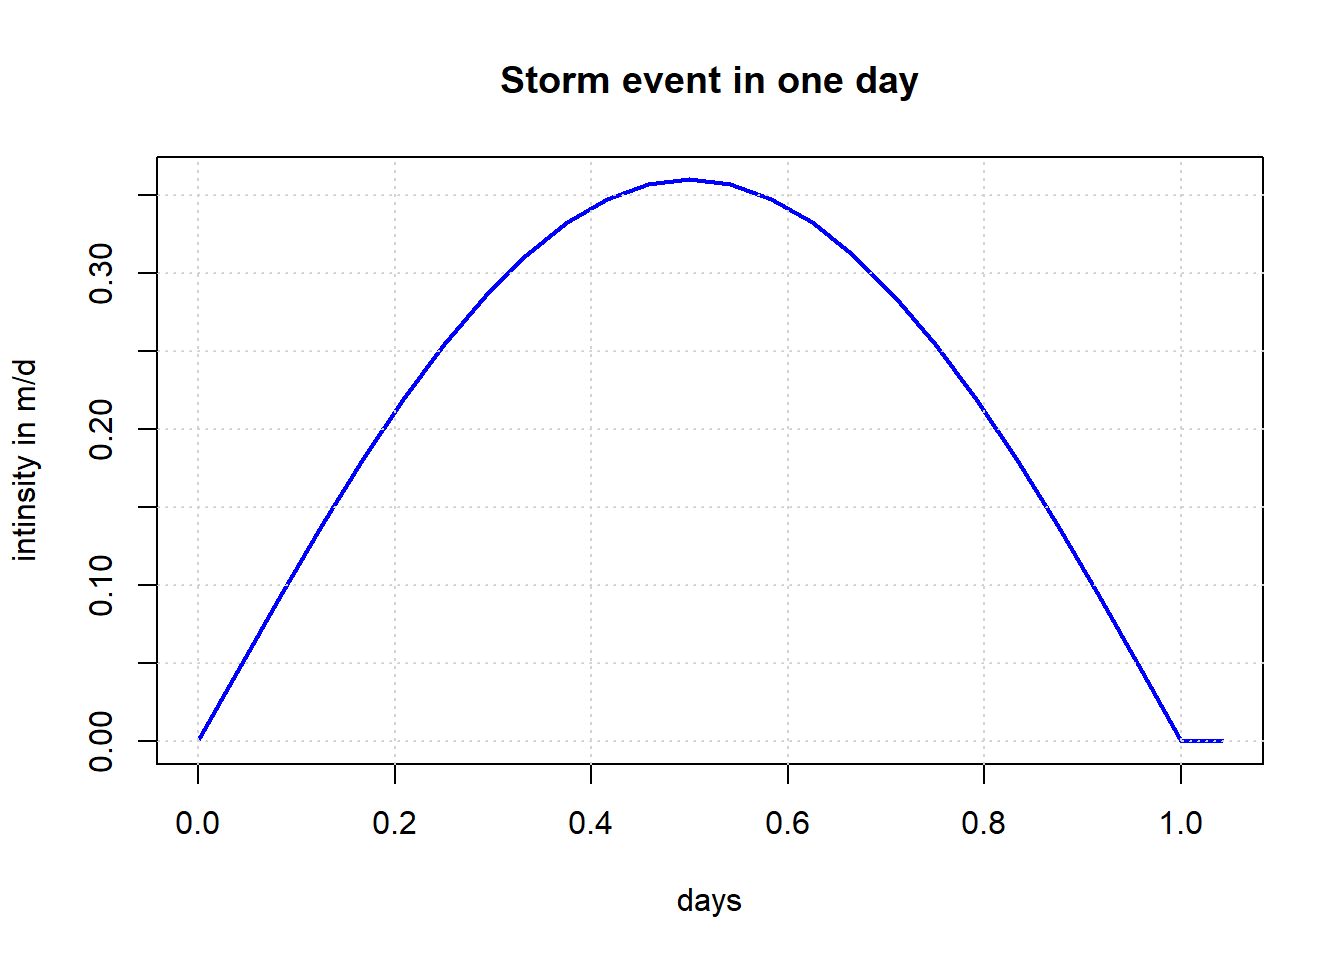
\includegraphics{start_Hooge_raam_coupling_files/figure-latex/unnamed-chunk-28-1.pdf}

\hypertarget{time-loop}{%
\subsection{Time loop}\label{time-loop}}

Finish the time loop replacing XXXX, YYYY, ZZZZ and AAAA.

\begin{Shaded}
\begin{Highlighting}[]
\CommentTok{\#data containers for results}
\NormalTok{GW.Q.trans }\OtherTok{=} \FunctionTok{c}\NormalTok{()}
\NormalTok{GW.H.trans }\OtherTok{=} \FunctionTok{c}\NormalTok{()}

\CommentTok{\#using the stationary head of the stationary model for the initial head for the first time step for the transient model}
\NormalTok{old.state }\OtherTok{=}\NormalTok{ XXXX}

\CommentTok{\#time aspects}
\NormalTok{delt.t }\OtherTok{=} \DecValTok{1}\SpecialCharTok{/}\DecValTok{24} \CommentTok{\# 1 hour}
\NormalTok{start.time }\OtherTok{=} \DecValTok{0}
\NormalTok{end.time }\OtherTok{=}  \FloatTok{10.0}

\NormalTok{current.time }\OtherTok{=}\NormalTok{ start.time}

\CommentTok{\#time loop}
\ControlFlowTok{while}\NormalTok{ (current.time }\SpecialCharTok{\textless{}}\NormalTok{ end.time)}
\NormalTok{\{}
\NormalTok{  current.time }\OtherTok{=}\NormalTok{ current.time }\SpecialCharTok{+}\NormalTok{ YYYY}
\NormalTok{  P }\OtherTok{=}\NormalTok{ ZZZZ}
  \FunctionTok{solve.steps}\NormalTok{(GW.trans)}
  \CommentTok{\#save intermediate data}
\NormalTok{  wb }\OtherTok{=} \FunctionTok{dataframe.balance}\NormalTok{(GW.trans)}
\NormalTok{  GW.Q.trans }\OtherTok{=} \FunctionTok{rbind}\NormalTok{(GW.Q.trans, }\FunctionTok{c}\NormalTok{(current.time,wb[}\DecValTok{2}\NormalTok{,}\DecValTok{3}\NormalTok{],wb[}\DecValTok{3}\NormalTok{,}\DecValTok{2}\NormalTok{],wb[}\DecValTok{3}\NormalTok{,}\DecValTok{3}\NormalTok{],wb[}\DecValTok{4}\NormalTok{,}\DecValTok{2}\NormalTok{],wb[}\DecValTok{5}\NormalTok{,}\DecValTok{3}\NormalTok{]))}
\NormalTok{  GW.H.trans }\OtherTok{=} \FunctionTok{rbind}\NormalTok{(GW.H.trans, }\FunctionTok{dataframe.states}\NormalTok{(GW.trans)[,}\DecValTok{2}\NormalTok{])}
  \CommentTok{\#save current state being the old state for the next time step}
\NormalTok{  old.state }\OtherTok{=}\NormalTok{ AAAA}
\NormalTok{\}}
  \CommentTok{\#storing and plotting results}
\NormalTok{  GW.Q.trans }\OtherTok{=} \FunctionTok{data.frame}\NormalTok{(GW.Q.trans)}
  \FunctionTok{colnames}\NormalTok{(GW.Q.trans) }\OtherTok{=} \FunctionTok{c}\NormalTok{(}\StringTok{"time"}\NormalTok{, }\StringTok{"surface\_runoff"}\NormalTok{,}\StringTok{"storage\_2flow"}\NormalTok{,}\StringTok{"storage\_2storage"}\NormalTok{,}\StringTok{"precip"}\NormalTok{,}\StringTok{"boundary"}\NormalTok{)}
  
  \CommentTok{\#plot some results}
\NormalTok{  Q.range }\OtherTok{=} \FunctionTok{range}\NormalTok{(GW.Q.trans}\SpecialCharTok{$}\NormalTok{surface\_runoff,GW.Q.trans}\SpecialCharTok{$}\NormalTok{storage\_2flow,GW.Q.trans}\SpecialCharTok{$}\NormalTok{storage\_2storage,GW.Q.trans}\SpecialCharTok{$}\NormalTok{precip,GW.Q.trans}\SpecialCharTok{$}\NormalTok{boundary)}
  \FunctionTok{plot}\NormalTok{(GW.Q.trans}\SpecialCharTok{$}\NormalTok{time,GW.Q.trans}\SpecialCharTok{$}\NormalTok{surface\_runoff,}\AttributeTok{ylim =}\NormalTok{ Q.range, }\AttributeTok{type =} \StringTok{"l"}\NormalTok{, }\AttributeTok{col =} \StringTok{"red"}\NormalTok{,}\AttributeTok{lwd =}\DecValTok{2}\NormalTok{,}
       \AttributeTok{ylab =} \StringTok{"flux rates in m2/d"}\NormalTok{, }\AttributeTok{xlab =} \StringTok{"time in days"}\NormalTok{, }\AttributeTok{main =} \StringTok{"flux rates groundwater model"}\NormalTok{)}
  \FunctionTok{lines}\NormalTok{(GW.Q.trans}\SpecialCharTok{$}\NormalTok{time,GW.Q.trans}\SpecialCharTok{$}\NormalTok{storage\_2flow,}\AttributeTok{col=}\StringTok{"yellow4"}\NormalTok{,}\AttributeTok{lwd =} \DecValTok{2}\NormalTok{)}
  \FunctionTok{lines}\NormalTok{(GW.Q.trans}\SpecialCharTok{$}\NormalTok{time,GW.Q.trans}\SpecialCharTok{$}\NormalTok{storage\_2storage,}\AttributeTok{col=}\StringTok{"orange"}\NormalTok{,}\AttributeTok{lwd =} \DecValTok{2}\NormalTok{)}
  \FunctionTok{lines}\NormalTok{(GW.Q.trans}\SpecialCharTok{$}\NormalTok{time,GW.Q.trans}\SpecialCharTok{$}\NormalTok{precip,}\AttributeTok{col=}\StringTok{"blue"}\NormalTok{, }\AttributeTok{lwd =} \DecValTok{2}\NormalTok{)}
  \FunctionTok{lines}\NormalTok{(GW.Q.trans}\SpecialCharTok{$}\NormalTok{time,GW.Q.trans}\SpecialCharTok{$}\NormalTok{boundary,}\AttributeTok{col=}\StringTok{"green"}\NormalTok{)}
  \FunctionTok{legend}\NormalTok{(}\StringTok{"topright"}\NormalTok{, }\AttributeTok{inset=}\NormalTok{.}\DecValTok{05}\NormalTok{,}
       \AttributeTok{legend=}\FunctionTok{c}\NormalTok{(}\StringTok{"runoff"}\NormalTok{,}\StringTok{"storage\_2flow"}\NormalTok{,}\StringTok{"storage\_2storage"}\NormalTok{,}\StringTok{"precipitation"}\NormalTok{,}\StringTok{"drainage"}\NormalTok{), }\AttributeTok{col=}\FunctionTok{c}\NormalTok{(}\StringTok{"red"}\NormalTok{,}\StringTok{"yellow4"}\NormalTok{,}\StringTok{"orange"}\NormalTok{,}\StringTok{"blue"}\NormalTok{,}\StringTok{"green"}\NormalTok{),}
       \AttributeTok{lwd=}\DecValTok{3}\NormalTok{,}\AttributeTok{horiz=}\ConstantTok{FALSE}\NormalTok{)}
\CommentTok{\#first 2 days 2*24 = 48 row}
  \FunctionTok{plot}\NormalTok{(GW.Q.trans}\SpecialCharTok{$}\NormalTok{time[}\DecValTok{1}\SpecialCharTok{:}\DecValTok{48}\NormalTok{],GW.Q.trans}\SpecialCharTok{$}\NormalTok{surface\_runoff[}\DecValTok{1}\SpecialCharTok{:}\DecValTok{48}\NormalTok{],}\AttributeTok{ylim =}\NormalTok{ Q.range, }\AttributeTok{type =} \StringTok{"o"}\NormalTok{, }\AttributeTok{col =} \StringTok{"red"}\NormalTok{,}\AttributeTok{lwd =}\DecValTok{2}\NormalTok{,}
       \AttributeTok{ylab =} \StringTok{"flux rates in m2/d"}\NormalTok{, }\AttributeTok{xlab =} \StringTok{"time in days"}\NormalTok{, }\AttributeTok{main =} \StringTok{"flux rates groundwater model"}\NormalTok{)}
  \FunctionTok{lines}\NormalTok{(GW.Q.trans}\SpecialCharTok{$}\NormalTok{time[}\DecValTok{1}\SpecialCharTok{:}\DecValTok{48}\NormalTok{],GW.Q.trans}\SpecialCharTok{$}\NormalTok{storage\_2flow[}\DecValTok{1}\SpecialCharTok{:}\DecValTok{48}\NormalTok{],}\AttributeTok{col=}\StringTok{"yellow4"}\NormalTok{,}\AttributeTok{lwd =} \DecValTok{2}\NormalTok{)}
  \FunctionTok{lines}\NormalTok{(GW.Q.trans}\SpecialCharTok{$}\NormalTok{time[}\DecValTok{1}\SpecialCharTok{:}\DecValTok{48}\NormalTok{],GW.Q.trans}\SpecialCharTok{$}\NormalTok{storage\_2storage[}\DecValTok{1}\SpecialCharTok{:}\DecValTok{48}\NormalTok{],}\AttributeTok{col=}\StringTok{"orange"}\NormalTok{,}\AttributeTok{lwd =} \DecValTok{2}\NormalTok{)}
  \FunctionTok{lines}\NormalTok{(GW.Q.trans}\SpecialCharTok{$}\NormalTok{time[}\DecValTok{1}\SpecialCharTok{:}\DecValTok{48}\NormalTok{],GW.Q.trans}\SpecialCharTok{$}\NormalTok{precip[}\DecValTok{1}\SpecialCharTok{:}\DecValTok{48}\NormalTok{],}\AttributeTok{col=}\StringTok{"blue"}\NormalTok{, }\AttributeTok{lwd =} \DecValTok{2}\NormalTok{)}
  \FunctionTok{lines}\NormalTok{(GW.Q.trans}\SpecialCharTok{$}\NormalTok{time[}\DecValTok{1}\SpecialCharTok{:}\DecValTok{48}\NormalTok{],GW.Q.trans}\SpecialCharTok{$}\NormalTok{boundary[}\DecValTok{1}\SpecialCharTok{:}\DecValTok{48}\NormalTok{],}\AttributeTok{col=}\StringTok{"green"}\NormalTok{, }\AttributeTok{lwd =} \DecValTok{2}\NormalTok{)}
  \FunctionTok{legend}\NormalTok{(}\StringTok{"topright"}\NormalTok{, }\AttributeTok{inset=}\NormalTok{.}\DecValTok{05}\NormalTok{,}
       \AttributeTok{legend=}\FunctionTok{c}\NormalTok{(}\StringTok{"runoff"}\NormalTok{,}\StringTok{"storage\_2flow"}\NormalTok{,}\StringTok{"storage\_2storage"}\NormalTok{,}\StringTok{"precipitation"}\NormalTok{,}\StringTok{"drainage"}\NormalTok{), }\AttributeTok{col=}\FunctionTok{c}\NormalTok{(}\StringTok{"red"}\NormalTok{,}\StringTok{"yellow4"}\NormalTok{,}\StringTok{"orange"}\NormalTok{,}\StringTok{"blue"}\NormalTok{,}\StringTok{"green"}\NormalTok{),}
       \AttributeTok{lwd=}\DecValTok{3}\NormalTok{,}\AttributeTok{horiz=}\ConstantTok{FALSE}\NormalTok{)}
\FunctionTok{grid}\NormalTok{()  }

\NormalTok{GW.Q.data }\OtherTok{=} \FunctionTok{summary}\NormalTok{(GW.Q.trans)  }
\NormalTok{knitr}\SpecialCharTok{::}\FunctionTok{kable}\NormalTok{(GW.Q.data, }\AttributeTok{caption =} \StringTok{"summary flow budget groundwater model in m2/d"}\NormalTok{, }\AttributeTok{format =} \StringTok{"simple"}\NormalTok{)}
\end{Highlighting}
\end{Shaded}

The term storage\_2flow stands for storage which is released to flow and
storage\_2storage is the amount of water which will be stored.

\hypertarget{part-3-coupling-open-water-and-groundwater}{%
\section{PART 3 Coupling open water and
groundwater}\label{part-3-coupling-open-water-and-groundwater}}

A ``loose'' coupling will be applied and analyzed. With this the open
water model will receive drainage and surface runoff fluxes from the
groundwater model.\\
Later on, one may use the calculated open water level to adjust the
drain depth in the groundwater model achieving a full coupling. This
will result in a full coupling: exchanging fluxes from groundwater to
open water and drain depth from open water to groundwater

\hypertarget{scaling-of-drainage-and-surface-runoff}{%
\subsubsection{Scaling of Drainage and surface
runoff}\label{scaling-of-drainage-and-surface-runoff}}

The pre-calculated drainage and surface runoff of the groundwater model
are used as input (``forcing'') for the open water model
\texttt{HR.backwatermodel} and need to be ``scaled'' to proper
dimensions; \(m^3/s\).\\
The groundwater drainage and surface runoff fluxes are based on one
typical parcel having an average ditch distance of 125 m. There are many
of these parcels in the catchment area of the Hooge Raam. These
discharge rates have unit \(m^2/d\) and need to be transformed to the
total discharging area of the Hooge Raam into units of \(m^3/s\). For
this, you can imagine all parcels, with an average ditch distance of
125m, were set behind each other resulting in a, let's call it a
\emph{diffuse length} calculated as:
\(\frac {\text{total_drained_area}}{\text{ditch_distance}}\). The figure
below illustrates the determination of the total diffuse length =
\({\sum\text{LocalPathLength}}=\frac{\text{Drained Area}}{\text{Ditch Distance}}\)\\
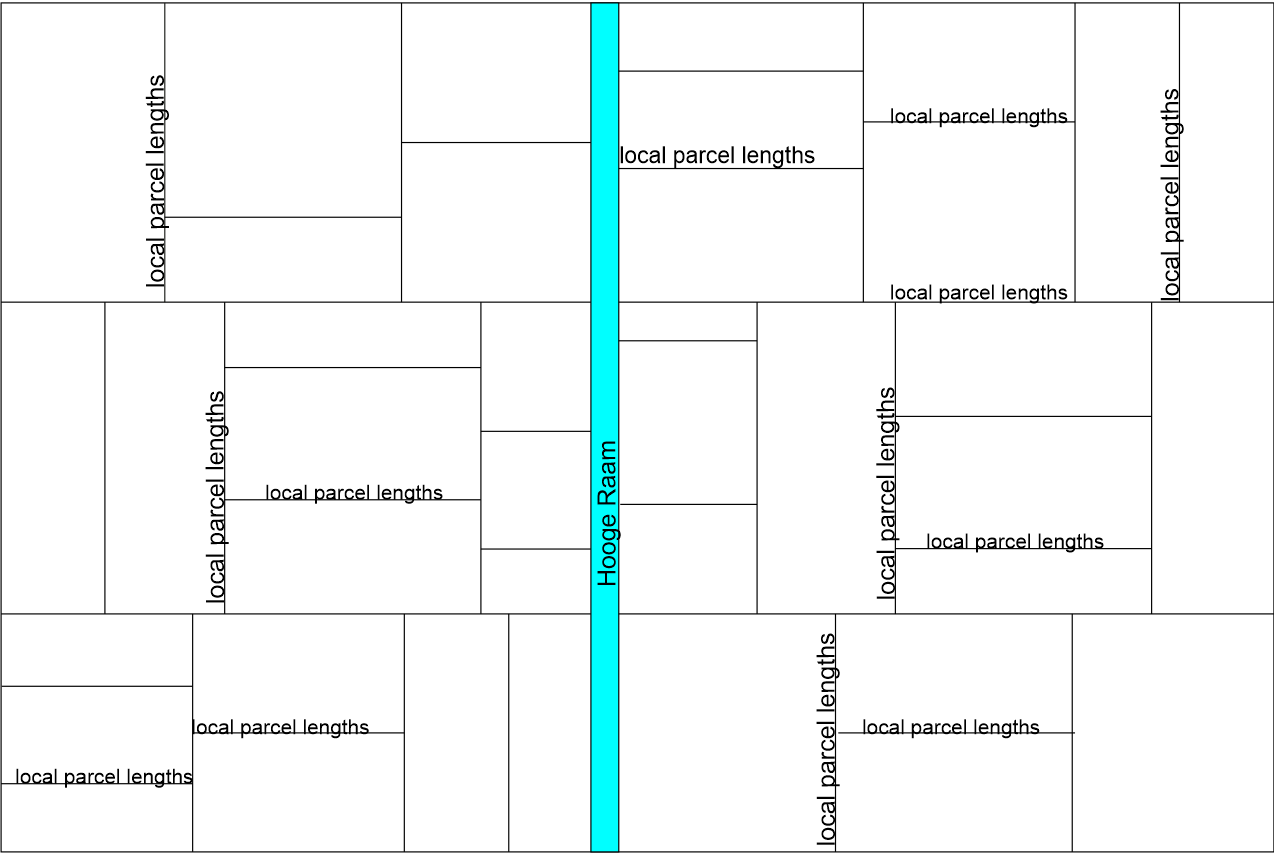
\includegraphics{Hooge_raam_diffuse_length.png}\\
Finally the groundwater drainage and surface runoff need to be
transformed to a lateral inflow rate of \(m^3/s/m_{HRcourse}\) for the
Hooge Raam.\\
The total considered discharging area of the Hooge Raam is 500 ha.

Determine the properly scaled drainage and runoff for the Hooge Raam
model ; \texttt{HR.backwatermodel}.

\begin{Shaded}
\begin{Highlighting}[]
\DocumentationTok{\#\# from groundwater discharge to lateral inflow into the Hooge Raam open water model}
\NormalTok{HR.discharge.area }\OtherTok{=}  \CommentTok{\#in m2}
\NormalTok{day2sec }\OtherTok{=} \DecValTok{86400} \CommentTok{\#from day to seconds}
\NormalTok{m2.day.to.m3.day }\OtherTok{=}\NormalTok{   HR.discharge.area}\SpecialCharTok{/}\NormalTok{L }\CommentTok{\#from m2/day to m3/day; a "diffuse length" based on the total drained area divided by the L(ditch distance)}

\NormalTok{Q.drainage.m3.d }\OtherTok{=} \CommentTok{\#}
\NormalTok{Q.drainage.m3.s }\OtherTok{=} \CommentTok{\#}
\NormalTok{Q.drainage.m2.s }\OtherTok{=} \CommentTok{\#}

\NormalTok{Q.runoff.m3.d }\OtherTok{=} \CommentTok{\#}
\NormalTok{Q.runoff.m3.s }\OtherTok{=} \CommentTok{\#}
\NormalTok{Q.runoff.m2.s }\OtherTok{=} \CommentTok{\#}
\end{Highlighting}
\end{Shaded}

Closely inspect the following chunk running the open water model
\texttt{HR.backwatermodel} with drainage and surface fluxes coming from
the groundwater model.

\begin{Shaded}
\begin{Highlighting}[]
\DocumentationTok{\#\#\#\#preparing open water model for drainage and surface runoff}
\FunctionTok{summary}\NormalTok{(HR.backwatermodel)}
\FunctionTok{plot}\NormalTok{(HR.backwatermodel,}\AttributeTok{fluxplot =}\NormalTok{ T)}

\DocumentationTok{\#\#removing the old lateral flux and adding the new drainage and runoff lateral fluxes}
\FunctionTok{rem.spatialflux}\NormalTok{(HR.backwatermodel,}\AttributeTok{name =} \StringTok{"drainage"}\NormalTok{)}
\FunctionTok{add.spatialflux}\NormalTok{(HR.backwatermodel,}\AttributeTok{rate =} \StringTok{"drainage"}\NormalTok{,}\AttributeTok{name =} \StringTok{"drainage"}\NormalTok{)}
\FunctionTok{add.spatialflux}\NormalTok{(HR.backwatermodel,}\AttributeTok{rate =} \StringTok{"runoff"}\NormalTok{, }\AttributeTok{name =} \StringTok{"runoff"}\NormalTok{)}
\FunctionTok{summary}\NormalTok{(HR.backwatermodel)}


\CommentTok{\#data containers for results}
\NormalTok{HR.Q.trans }\OtherTok{=} \FunctionTok{c}\NormalTok{()}
\NormalTok{HR.h.trans }\OtherTok{=} \FunctionTok{c}\NormalTok{()}
\NormalTok{HR.Q\_upstream }\OtherTok{=} \FunctionTok{c}\NormalTok{()}
\NormalTok{HR.Q\_downstream }\OtherTok{=} \FunctionTok{c}\NormalTok{()}
\CommentTok{\#data container for results}

\CommentTok{\#plot facility}
\FunctionTok{plot}\NormalTok{(nodes,}\FunctionTok{HR.zb}\NormalTok{(nodes),}\AttributeTok{col=}\StringTok{"brown"}\NormalTok{,}\AttributeTok{type=}\StringTok{"l"}\NormalTok{,}\AttributeTok{lwd=}\DecValTok{4}\NormalTok{,}\AttributeTok{ylim=}\FunctionTok{c}\NormalTok{(}\DecValTok{11}\NormalTok{,}\DecValTok{18}\NormalTok{),}
     \AttributeTok{xlab=}\StringTok{"l"}\NormalTok{,}\AttributeTok{ylab=}\StringTok{"h"}\NormalTok{,}\AttributeTok{main=}\FunctionTok{paste}\NormalTok{(}\StringTok{"Transient water levels Hooge Raam"}\NormalTok{))}
\FunctionTok{lines}\NormalTok{(}\FunctionTok{dataframe.states}\NormalTok{(HR.backwatermodel), }\AttributeTok{col =} \StringTok{"blue"}\NormalTok{, }\AttributeTok{lwd =} \DecValTok{3}\NormalTok{)}
\FunctionTok{grid}\NormalTok{()}

\CommentTok{\#delt.t = 1/24 comes from groundwater model}
\NormalTok{current.time }\OtherTok{=} \FloatTok{0.0}
\CommentTok{\#end.time = 2 comes from groundwater model}
\NormalTok{time.step }\OtherTok{=} \DecValTok{0}

\DocumentationTok{\#\#\#\#time loop for HR.backwatermodel with fluxes from the groundwater model}
\ControlFlowTok{while}\NormalTok{(current.time }\SpecialCharTok{\textless{}}\NormalTok{ end.time)}

\NormalTok{\{}
\NormalTok{  current.time }\OtherTok{=}\NormalTok{ current.time }\SpecialCharTok{+}\NormalTok{ delt.t}
\NormalTok{  time.step }\OtherTok{=}\NormalTok{ time.step }\SpecialCharTok{+} \DecValTok{1}
\NormalTok{  drainage }\OtherTok{=}\NormalTok{ Q.drainage.m2.s[time.step]}
\NormalTok{  runoff }\OtherTok{=}\NormalTok{ Q.runoff.m2.s[time.step]}
  \FunctionTok{solve.steps}\NormalTok{(HR.backwatermodel)}
  \DocumentationTok{\#\#saving intermediate results}
\NormalTok{  wb }\OtherTok{=} \FunctionTok{dataframe.balance}\NormalTok{(HR.backwatermodel)}
\NormalTok{  HR.Q.trans }\OtherTok{=} \FunctionTok{rbind}\NormalTok{(HR.Q.trans, }\FunctionTok{c}\NormalTok{(current.time,wb[}\DecValTok{4}\NormalTok{,}\DecValTok{2}\NormalTok{],wb[}\DecValTok{3}\NormalTok{,}\DecValTok{2}\NormalTok{],wb[}\DecValTok{2}\NormalTok{,}\DecValTok{2}\NormalTok{],wb[}\DecValTok{4}\NormalTok{,}\DecValTok{3}\NormalTok{]))}
\NormalTok{  HR.h.trans }\OtherTok{=} \FunctionTok{rbind}\NormalTok{(HR.h.trans, }\FunctionTok{dataframe.states}\NormalTok{(HR.backwatermodel)[,}\DecValTok{2}\NormalTok{])}
  
  \CommentTok{\#create plot to generate an animation in the knitted HTML document}
  \FunctionTok{plot}\NormalTok{(nodes,}\FunctionTok{HR.zb}\NormalTok{(nodes),}\AttributeTok{col=}\StringTok{"brown"}\NormalTok{,}\AttributeTok{type=}\StringTok{"l"}\NormalTok{,}\AttributeTok{lwd=}\DecValTok{4}\NormalTok{,}\AttributeTok{ylim=}\FunctionTok{c}\NormalTok{(}\DecValTok{11}\NormalTok{,}\DecValTok{18}\NormalTok{),}
       \AttributeTok{xlab=}\StringTok{"l"}\NormalTok{,}\AttributeTok{ylab=}\StringTok{"h"}\NormalTok{,}\AttributeTok{main=}\FunctionTok{paste}\NormalTok{(}\StringTok{"Transient water levels Hooge Raam"}\NormalTok{))}
  \FunctionTok{lines}\NormalTok{(}\FunctionTok{dataframe.states}\NormalTok{(HR.backwatermodel), }\AttributeTok{col =} \StringTok{"blue"}\NormalTok{, }\AttributeTok{lwd =} \DecValTok{3}\NormalTok{)}
  \FunctionTok{grid}\NormalTok{()}
  
\NormalTok{\}}
  \DocumentationTok{\#\# creating data frames for the result of the open water model with drainage and surface runoff }
\NormalTok{ HR.Q.trans }\OtherTok{=} \FunctionTok{data.frame}\NormalTok{(HR.Q.trans)}
 \FunctionTok{colnames}\NormalTok{(HR.Q.trans) }\OtherTok{=} \FunctionTok{c}\NormalTok{(}\StringTok{"time"}\NormalTok{,}\StringTok{"boundary\_upstream"}\NormalTok{,}\StringTok{"runoff"}\NormalTok{,}\StringTok{"drainage"}\NormalTok{,}\StringTok{"boundary\_downstream"}\NormalTok{)}
\NormalTok{ HR.h.trans }\OtherTok{=} \FunctionTok{data.frame}\NormalTok{(HR.h.trans)}
\end{Highlighting}
\end{Shaded}

\hypertarget{checking-fluxes-and-total-volumes}{%
\subsubsection{Checking fluxes and total
volumes}\label{checking-fluxes-and-total-volumes}}

For both the transient groundwater and the pseudo-stationary open water
model the total volumes of water (in \(m^3\)) during the simulation time
are compared with both models.

\hypertarget{groundwater}{%
\paragraph{groundwater}\label{groundwater}}

Volume balance for the groundwater model \[
Total_{in} = \sum_{t= 0}^{t=T}Precip(t)\Delta t\\
Total_{out} = \left \{ \sum_{t=0}^{t=T} Qsto(t)+\sum_{t=0}^{t=T} Runoff(t) + \sum_{t=0}^{t=T} Drainage(t) \right \} \Delta t
\] Recall that the water balance of the groundwater model is expressed
in \(m^2/d\). To come to volumes (\(m^3\)) one need to consider the
``diffuse length'' and the time step.

\begin{Shaded}
\begin{Highlighting}[]
\CommentTok{\# Water volumes for the 1D groundwater model during the total simulation time}

\NormalTok{GW.volume.drainage }\OtherTok{=} \FunctionTok{sum}\NormalTok{(GW.Q.trans}\SpecialCharTok{$}\NormalTok{boundary) }\SpecialCharTok{*}\NormalTok{ m2.day.to.m3.day }\SpecialCharTok{*}\NormalTok{ delt.t}
\NormalTok{GW.volume.runoff }\OtherTok{=} \FunctionTok{sum}\NormalTok{(GW.Q.trans}\SpecialCharTok{$}\NormalTok{surface\_runoff) }\SpecialCharTok{*}\NormalTok{ m2.day.to.m3.day }\SpecialCharTok{*}\NormalTok{ delt.t}

\NormalTok{GW.volume.storage\_into }\OtherTok{=} \FunctionTok{sum}\NormalTok{(GW.Q.trans}\SpecialCharTok{$}\NormalTok{storage\_2flow) }\SpecialCharTok{*}\NormalTok{ m2.day.to.m3.day }\SpecialCharTok{*}\NormalTok{ delt.t}
\NormalTok{GW.volume.storage\_outof }\OtherTok{=} \FunctionTok{sum}\NormalTok{(GW.Q.trans}\SpecialCharTok{$}\NormalTok{storage\_2storage) }\SpecialCharTok{*}\NormalTok{ m2.day.to.m3.day }\SpecialCharTok{*}\NormalTok{ delt.t}

\NormalTok{GW.volume.precipitation }\OtherTok{=} \FunctionTok{sum}\NormalTok{(GW.Q.trans}\SpecialCharTok{$}\NormalTok{precip) }\SpecialCharTok{*}\NormalTok{ m2.day.to.m3.day }\SpecialCharTok{*}\NormalTok{ delt.t}

\NormalTok{GW.misfit }\OtherTok{=}\NormalTok{ GW.volume.precipitation }\SpecialCharTok{{-}}\NormalTok{ GW.volume.drainage }\SpecialCharTok{{-}}\NormalTok{ GW.volume.runoff }\SpecialCharTok{{-}}\NormalTok{ GW.volume.storage\_outof }\SpecialCharTok{+}\NormalTok{ GW.volume.storage\_into}

\NormalTok{volume.bal.GW }\OtherTok{=} \FunctionTok{data.frame}\NormalTok{(}\AttributeTok{Groundwater =} \FunctionTok{c}\NormalTok{(}\StringTok{"precipitation"}\NormalTok{,}\StringTok{"storage\_2flow"}\NormalTok{,}\StringTok{"drainage"}\NormalTok{,}\StringTok{"runoff"}\NormalTok{,}\StringTok{"storage\_2storage"}\NormalTok{,}\StringTok{"total"}\NormalTok{),}
                        \AttributeTok{Volume\_in =} \FunctionTok{c}\NormalTok{(GW.volume.precipitation,GW.volume.storage\_into,}\DecValTok{0}\NormalTok{,}\DecValTok{0}\NormalTok{,}\DecValTok{0}\NormalTok{,}\FunctionTok{sum}\NormalTok{(GW.volume.precipitation,GW.volume.storage\_into)),}
                        \AttributeTok{Volume\_out =} \FunctionTok{c}\NormalTok{(}\DecValTok{0}\NormalTok{,}\DecValTok{0}\NormalTok{,GW.volume.drainage,GW.volume.runoff,GW.volume.storage\_outof,}\FunctionTok{sum}\NormalTok{(GW.volume.drainage,GW.volume.runoff,GW.volume.storage\_outof)))}\CommentTok{\#,}
                        
\NormalTok{knitr}\SpecialCharTok{::}\FunctionTok{kable}\NormalTok{(volume.bal.GW,}\AttributeTok{format =} \StringTok{"simple"}\NormalTok{, }\AttributeTok{caption =} \StringTok{"Total volumes in m\^{}3 groundwater model"}\NormalTok{)}
\end{Highlighting}
\end{Shaded}

\hypertarget{open-water}{%
\paragraph{open water}\label{open-water}}

\[
Total_{in} = \sum_{t=0}^{t=T} boundary_{upstream}\Delta t + \sum_{t=0}^{t=T} runoff \Delta t + \sum_{t=0}^{t=T} drainage \Delta t\\
Total_{out} = \sum_{t=0}^{t=T} boundary_{downstream}
\]

\begin{Shaded}
\begin{Highlighting}[]
\CommentTok{\# water volumes for the 1D open water (Hooge Raam) model during the total simulation time}
\NormalTok{HR.volume.bnd.upstream }\OtherTok{=} \FunctionTok{sum}\NormalTok{(HR.Q.trans}\SpecialCharTok{$}\NormalTok{boundary\_upstream) }\SpecialCharTok{*}\NormalTok{ delt.t }\SpecialCharTok{*} \DecValTok{86400} \CommentTok{\#unit delt.t is in days!}
\NormalTok{HR.volume.runoff }\OtherTok{=} \FunctionTok{sum}\NormalTok{(HR.Q.trans}\SpecialCharTok{$}\NormalTok{runoff) }\SpecialCharTok{*}\NormalTok{ delt.t }\SpecialCharTok{*} \DecValTok{86400}
\NormalTok{HR.volume.drainage }\OtherTok{=} \FunctionTok{sum}\NormalTok{(HR.Q.trans}\SpecialCharTok{$}\NormalTok{drainage) }\SpecialCharTok{*}\NormalTok{ delt.t }\SpecialCharTok{*} \DecValTok{86400}
\NormalTok{HR.volume.bnd.downstream }\OtherTok{=} \FunctionTok{sum}\NormalTok{(HR.Q.trans}\SpecialCharTok{$}\NormalTok{boundary\_downstream) }\SpecialCharTok{*}\NormalTok{ delt.t }\SpecialCharTok{*} \DecValTok{86400}

\NormalTok{HR.volume.in }\OtherTok{=}\NormalTok{ HR.volume.bnd.upstream }\SpecialCharTok{+}\NormalTok{ HR.volume.runoff }\SpecialCharTok{+}\NormalTok{ HR.volume.drainage}
\NormalTok{HR.volume.out }\OtherTok{=}\NormalTok{ HR.volume.bnd.downstream}


\DocumentationTok{\#\# this should add up to the total amount of precipitation during the simulation time.}

\NormalTok{volume.bal.HR }\OtherTok{=} \FunctionTok{data.frame}\NormalTok{(}\AttributeTok{Open\_water =} \FunctionTok{c}\NormalTok{(}\StringTok{"inflow\_upstream"}\NormalTok{,}\StringTok{"surface\_runoff"}\NormalTok{,}\StringTok{"drainage"}\NormalTok{,}\StringTok{"outflow\_downstream"}\NormalTok{,}\StringTok{"total"}\NormalTok{),}
                           \AttributeTok{Volume\_in =} \FunctionTok{c}\NormalTok{(HR.volume.bnd.upstream,HR.volume.runoff,HR.volume.drainage,}\DecValTok{0}\NormalTok{,HR.volume.in),}
                           \AttributeTok{Volume\_out =} \FunctionTok{c}\NormalTok{(}\DecValTok{0}\NormalTok{,}\DecValTok{0}\NormalTok{,}\DecValTok{0}\NormalTok{,HR.volume.bnd.downstream,HR.volume.out))}
\NormalTok{knitr}\SpecialCharTok{::}\FunctionTok{kable}\NormalTok{(volume.bal.HR,}\AttributeTok{format.arg =} \FunctionTok{list}\NormalTok{(}\AttributeTok{digits =} \DecValTok{8}\NormalTok{,}\AttributeTok{nsmall =} \DecValTok{3}\NormalTok{), }\AttributeTok{caption =} \StringTok{"Total volumes in m\^{}3 open water model"}\NormalTok{) }\CommentTok{\#,digits = 15)}
\end{Highlighting}
\end{Shaded}

Check whether the output of the groundwater are the same inputs for the
open water model.

\hypertarget{time-series-analysis}{%
\subsection{Time series analysis}\label{time-series-analysis}}

It can be interesting to for example compare time series for the
precipitation and discharge of the Hooge Raam. With this, one can
examine the response of a storm event on the open water - groundwater
system.

\begin{Shaded}
\begin{Highlighting}[]
\FunctionTok{plot}\NormalTok{(GW.Q.trans}\SpecialCharTok{$}\NormalTok{time, }\FunctionTok{P.pattern}\NormalTok{(GW.Q.trans}\SpecialCharTok{$}\NormalTok{time), }\AttributeTok{col =} \StringTok{"blue"}\NormalTok{, }\AttributeTok{lwd =}\DecValTok{2}\NormalTok{, }\AttributeTok{ylab =} \StringTok{"m/d"}\NormalTok{,}\AttributeTok{xlab =} \StringTok{"days"}\NormalTok{,}\AttributeTok{type=} \StringTok{"l"}\NormalTok{, }\AttributeTok{main =} \StringTok{"Transient fluxes open water model in m/d"}\NormalTok{, }\AttributeTok{sub =} \StringTok{"Total simulation time"}\NormalTok{)}
\NormalTok{HR.discharge.m.d }\OtherTok{=}\NormalTok{ HR.Q.trans}\SpecialCharTok{$}\NormalTok{boundary\_downstream }\SpecialCharTok{*} \DecValTok{86400} \SpecialCharTok{/}\NormalTok{ HR.discharge.area}
\FunctionTok{lines}\NormalTok{(HR.Q.trans}\SpecialCharTok{$}\NormalTok{time,HR.discharge.m.d,}\AttributeTok{col =} \StringTok{"red"}\NormalTok{, }\AttributeTok{lwd =}\DecValTok{2}\NormalTok{)}
\NormalTok{HR.runoff.m.d }\OtherTok{=}\NormalTok{ HR.Q.trans}\SpecialCharTok{$}\NormalTok{runoff }\SpecialCharTok{*} \DecValTok{86400} \SpecialCharTok{/}\NormalTok{ HR.discharge.area}
\FunctionTok{lines}\NormalTok{(HR.Q.trans}\SpecialCharTok{$}\NormalTok{time,HR.runoff.m.d, }\AttributeTok{col =} \StringTok{"brown"}\NormalTok{,}\AttributeTok{lwd =}  \DecValTok{2}\NormalTok{)}
\NormalTok{HR.drainage.m.d }\OtherTok{=}\NormalTok{ HR.Q.trans}\SpecialCharTok{$}\NormalTok{drainage }\SpecialCharTok{*} \DecValTok{86400} \SpecialCharTok{/}\NormalTok{ HR.discharge.area}
\FunctionTok{lines}\NormalTok{(HR.Q.trans}\SpecialCharTok{$}\NormalTok{time,HR.drainage.m.d, }\AttributeTok{col =} \StringTok{"green"}\NormalTok{,}\AttributeTok{lwd =}\DecValTok{2}\NormalTok{)}
\FunctionTok{grid}\NormalTok{()}
\FunctionTok{legend}\NormalTok{(}\StringTok{"topright"}\NormalTok{, }\AttributeTok{inset=}\NormalTok{.}\DecValTok{05}\NormalTok{,}
       \AttributeTok{legend=}\FunctionTok{c}\NormalTok{(}\StringTok{"precipitation"}\NormalTok{,}\StringTok{"HR discharge"}\NormalTok{,}\StringTok{"runoff"}\NormalTok{,}\StringTok{"drainage"}\NormalTok{), }\AttributeTok{col=}\FunctionTok{c}\NormalTok{(}\StringTok{"blue"}\NormalTok{,}\StringTok{"red"}\NormalTok{,}\StringTok{"brown"}\NormalTok{,}\StringTok{"green"}\NormalTok{),}
       \AttributeTok{lwd=}\DecValTok{3}\NormalTok{,}\AttributeTok{horiz=}\ConstantTok{FALSE}\NormalTok{)}

\NormalTok{time.max.precip }\OtherTok{=} \FunctionTok{which.max}\NormalTok{(}\FunctionTok{P.pattern}\NormalTok{(GW.Q.trans}\SpecialCharTok{$}\NormalTok{time))}\SpecialCharTok{*}\NormalTok{delt.t}
\FunctionTok{abline}\NormalTok{(}\AttributeTok{v=}\NormalTok{time.max.precip, }\AttributeTok{col =} \StringTok{"blue"}\NormalTok{)}

\NormalTok{time.max.discharge }\OtherTok{=} \FunctionTok{which.max}\NormalTok{(HR.Q.trans}\SpecialCharTok{$}\NormalTok{boundary\_downstream)}\SpecialCharTok{*}\NormalTok{delt.t}
\NormalTok{time.max.runoff }\OtherTok{=} \FunctionTok{which.max}\NormalTok{(HR.Q.trans}\SpecialCharTok{$}\NormalTok{runoff)}\SpecialCharTok{*}\NormalTok{delt.t}
\NormalTok{time.max.drainage }\OtherTok{=} \FunctionTok{which.max}\NormalTok{(HR.Q.trans}\SpecialCharTok{$}\NormalTok{drainage)}\SpecialCharTok{*}\NormalTok{delt.t}

\FunctionTok{abline}\NormalTok{(}\AttributeTok{v=}\NormalTok{time.max.discharge,}\AttributeTok{col=}\StringTok{\textquotesingle{}red\textquotesingle{}}\NormalTok{,}\AttributeTok{lwd=}\DecValTok{3}\NormalTok{)}
\FunctionTok{abline}\NormalTok{(}\AttributeTok{v=}\NormalTok{time.max.drainage, }\AttributeTok{col =} \StringTok{"green"}\NormalTok{)}
\end{Highlighting}
\end{Shaded}

Zooming in for the first two days.

\begin{Shaded}
\begin{Highlighting}[]
\NormalTok{plot.time }\OtherTok{=}\NormalTok{ GW.Q.trans}\SpecialCharTok{$}\NormalTok{time[}\DecValTok{1}\SpecialCharTok{:}\DecValTok{48}\NormalTok{]}
\FunctionTok{plot}\NormalTok{(plot.time, }\FunctionTok{P.pattern}\NormalTok{(plot.time), }\AttributeTok{col =} \StringTok{"blue"}\NormalTok{, }\AttributeTok{lwd =}\DecValTok{2}\NormalTok{, }\AttributeTok{ylab =} \StringTok{"m/d"}\NormalTok{,}\AttributeTok{xlab =} \StringTok{"days"}\NormalTok{,}\AttributeTok{type=} \StringTok{"o"}\NormalTok{, }\AttributeTok{main =} \StringTok{"Transient fluxes open water model in m/d"}\NormalTok{, }\AttributeTok{sub =} \StringTok{"First two days simulation time"}\NormalTok{)}
\NormalTok{HR.discharge.m.d }\OtherTok{=}\NormalTok{ HR.Q.trans}\SpecialCharTok{$}\NormalTok{boundary\_downstream }\SpecialCharTok{*} \DecValTok{86400} \SpecialCharTok{/}\NormalTok{ HR.discharge.area}
\FunctionTok{lines}\NormalTok{(HR.Q.trans}\SpecialCharTok{$}\NormalTok{time,HR.discharge.m.d,}\AttributeTok{col =} \StringTok{"red"}\NormalTok{, }\AttributeTok{lwd =}\DecValTok{2}\NormalTok{)}
\NormalTok{HR.runoff.m.d }\OtherTok{=}\NormalTok{ HR.Q.trans}\SpecialCharTok{$}\NormalTok{runoff }\SpecialCharTok{*} \DecValTok{86400} \SpecialCharTok{/}\NormalTok{ HR.discharge.area}
\FunctionTok{lines}\NormalTok{(HR.Q.trans}\SpecialCharTok{$}\NormalTok{time,HR.runoff.m.d, }\AttributeTok{col =} \StringTok{"brown"}\NormalTok{,}\AttributeTok{lwd =}  \DecValTok{2}\NormalTok{)}
\NormalTok{HR.drainage.m.d }\OtherTok{=}\NormalTok{ HR.Q.trans}\SpecialCharTok{$}\NormalTok{drainage }\SpecialCharTok{*} \DecValTok{86400} \SpecialCharTok{/}\NormalTok{ HR.discharge.area}
\FunctionTok{lines}\NormalTok{(HR.Q.trans}\SpecialCharTok{$}\NormalTok{time,HR.drainage.m.d, }\AttributeTok{col =} \StringTok{"green"}\NormalTok{,}\AttributeTok{lwd =}\DecValTok{2}\NormalTok{)}
\FunctionTok{grid}\NormalTok{()}
\FunctionTok{legend}\NormalTok{(}\StringTok{"topright"}\NormalTok{, }\AttributeTok{inset=}\NormalTok{.}\DecValTok{05}\NormalTok{,}
       \AttributeTok{legend=}\FunctionTok{c}\NormalTok{(}\StringTok{"precipitation"}\NormalTok{,}\StringTok{"HR discharge"}\NormalTok{,}\StringTok{"runoff"}\NormalTok{,}\StringTok{"drainage"}\NormalTok{), }\AttributeTok{col=}\FunctionTok{c}\NormalTok{(}\StringTok{"blue"}\NormalTok{,}\StringTok{"red"}\NormalTok{,}\StringTok{"brown"}\NormalTok{,}\StringTok{"green"}\NormalTok{),}
       \AttributeTok{lwd=}\DecValTok{3}\NormalTok{,}\AttributeTok{horiz=}\ConstantTok{FALSE}\NormalTok{)}

\NormalTok{time.max.precip }\OtherTok{=} \FunctionTok{which.max}\NormalTok{(}\FunctionTok{P.pattern}\NormalTok{(plot.time))}\SpecialCharTok{*}\NormalTok{delt.t}
\FunctionTok{abline}\NormalTok{(}\AttributeTok{v=}\NormalTok{time.max.precip, }\AttributeTok{col =} \StringTok{"blue"}\NormalTok{)}

\NormalTok{time.max.discharge }\OtherTok{=} \FunctionTok{which.max}\NormalTok{(HR.Q.trans}\SpecialCharTok{$}\NormalTok{boundary\_downstream)}\SpecialCharTok{*}\NormalTok{delt.t}
\NormalTok{time.max.runoff }\OtherTok{=} \FunctionTok{which.max}\NormalTok{(HR.Q.trans}\SpecialCharTok{$}\NormalTok{runoff)}\SpecialCharTok{*}\NormalTok{delt.t}
\NormalTok{time.max.drainage }\OtherTok{=} \FunctionTok{which.max}\NormalTok{(HR.Q.trans}\SpecialCharTok{$}\NormalTok{drainage)}\SpecialCharTok{*}\NormalTok{delt.t}

\FunctionTok{abline}\NormalTok{(}\AttributeTok{v=}\NormalTok{time.max.discharge,}\AttributeTok{col=}\StringTok{\textquotesingle{}red\textquotesingle{}}\NormalTok{,}\AttributeTok{lwd=}\DecValTok{1}\NormalTok{)}
\FunctionTok{abline}\NormalTok{(}\AttributeTok{v=}\NormalTok{time.max.drainage, }\AttributeTok{col =} \StringTok{"green"}\NormalTok{)}
\end{Highlighting}
\end{Shaded}

From the graphs it's clearly visible that the discharge is delayed
compared to the precipitation. The max. precipitation is at day
\texttt{time.max.precip} (blue vertical line) and the max. discharge is
at day : \texttt{time.max.discharge} (red vertical line)

The moment when the maximum discharge at the weir of the Hooge Raam is
reached coincides with the max. runoff. Why? ANSWER: Runoff and drainage
both come from the same 1D groundwater model. Since this model is 1
dimensional, from ditch to ditch, it does not contain a spatial
distribution with parcel far away and close by the Hooge Raam. Moreover
the 1D transient groundwater model calculates the effect of
precipitation on groundwater storage, drainage and surface runoff in the
same time step. In other words, precipitation is distributed over these
three groundwater sinks in the same time.

\hypertarget{part-4-sensitivity-analysis}{%
\section{PART 4 Sensitivity
analysis}\label{part-4-sensitivity-analysis}}

Here we will consider the local sensitivity analysis.

The task is to determine what the uncertainty of a model (derived)
result is due to the used the parameter values in the model.

For example; suppose one want's to determine the uncertainty of the max
head in a groundwater model, due to the model parameters (like kD,
boundary-conditions, precipitation, for which you not have exact, or
good values.

For this the following aspects need to be considered/determined:

\begin{enumerate}
\def\labelenumi{\arabic{enumi}.}
\item
  derived result, like the max discharge (in time) of the Hooge Raam
\item
  list of parameters and it optimal (assumed) values
\item
  list of the scale of variation of the parameters
\item
  local sensitivities for the parameters
\item
  scaled contributions to uncertainty of each parameter
\end{enumerate}

\hypertarget{derived-result}{%
\subsection{Derived result}\label{derived-result}}

all results of the current coupled models:

\hypertarget{groundwater-model}{%
\subsubsection{groundwater model:}\label{groundwater-model}}

\begin{enumerate}
\def\labelenumi{\arabic{enumi}.}
\item
  heads, \(H\), at different time steps and locations
\item
  water balance terms(for different time steps and locations:

  \begin{enumerate}
  \def\labelenumii{\arabic{enumii}.}
  \item
    boundary in, boundary out (drainage)
  \item
    internal flux
  \item
    storage
  \item
    precipitation
  \item
    surface runoff
  \end{enumerate}
\end{enumerate}

The max discharge is
\texttt{HR.Q.trans\$boundary\_downstream{[}time.max.discharge{]}} in
\(m^3/s\) and takes place at time :
\texttt{HR.Q.trans\$time{[}time.max.discharge{]}} days.

\hypertarget{open-water-model}{%
\subsubsection{open water model:}\label{open-water-model}}

\begin{enumerate}
\def\labelenumi{\arabic{enumi}.}
\item
  water levels at different time steps and locations
\item
  water balance terms (for different time steps and locations)

  \begin{enumerate}
  \def\labelenumii{\arabic{enumii}.}
  \item
    influx upstream
  \item
    outflux downstream
  \end{enumerate}
\end{enumerate}

\hypertarget{parameter-list}{%
\subsection{Parameter list}\label{parameter-list}}

All parameters can be used for analysis of the uncertainty of the model
result, of \textbf{both}, models.

\hypertarget{groundwater-model-1}{%
\subsubsection{groundwater model:}\label{groundwater-model-1}}

\begin{enumerate}
\def\labelenumi{\arabic{enumi}.}
\item
  Transmissivity of the subsoil \texttt{GW.kD}
\item
  Entrance resistance of the ditch \texttt{C\_ditch}
\item
  Average drain level of the area \texttt{H\_drainage}
\item
  Vertical resistance top layer soil \texttt{C\_surface}
\item
  Average surface level drainage system \texttt{H\_surface}
\item
  Storage coefficient; \texttt{GW.S}
\end{enumerate}

\hypertarget{open-water-model-1}{%
\subsubsection{open water model:}\label{open-water-model-1}}

\begin{enumerate}
\def\labelenumi{\arabic{enumi}.}
\item
  value weir constant (currently \texttt{1.83})
\item
  Weir crest height \texttt{HR.weir.crest}
\item
  Weir width \texttt{HR.weir.width}
\item
  Manning coefficient \texttt{HR.n}
\item
  River width \texttt{HR.b}
\item
  Side slopes \texttt{HR.m}
\end{enumerate}

\hypertarget{scale-of-variation-sigma}{%
\subsection{\texorpdfstring{Scale of variation
(\(\sigma\))}{Scale of variation (\textbackslash sigma)}}\label{scale-of-variation-sigma}}

The scale of variation could be based on literature, field experiments
or for example on a model calibration.

\hypertarget{calculation-local-sensitivities}{%
\subsection{Calculation local
sensitivities}\label{calculation-local-sensitivities}}

After we have determined the base model result, we will determine the
local sensitivity of the base result w.r.t. parameter;
\(\frac{\partial Model_{result}}{\partial P_i}\).

\hypertarget{scaled-contributions-to-result-uncertainty}{%
\subsection{Scaled contributions to result
uncertainty}\label{scaled-contributions-to-result-uncertainty}}

\hypertarget{assignment}{%
\subsection{ASSIGNMENT}\label{assignment}}

Carry out a local sensitivity analysis for one of the model results, the
groundwater and open water model.

\begin{enumerate}
\def\labelenumi{\arabic{enumi}.}
\tightlist
\item
  Choose at least 6 parameters, preferably from both models, to carry
  out the sensitivity analysis with
\item
  Estimate the scale of variation of these parameters, based on your
  experience, what you have heard during courses or simply google it
\item
  Create chunks to determine the local sensitivities
\item
  Make use of the pre-programmed \texttt{sensitivity.loop()} executing
  time loops for each model and saving intermediate data
\item
  Create a chunk to calculate the derived uncertainties
\end{enumerate}

This sensitivity.loop() contains many lines of code but basically does
the following:

\begin{enumerate}
\def\labelenumi{\arabic{enumi}.}
\tightlist
\item
  Run the transient groundwater model
\item
  Store results, flux rates (m2/d) and heads, of the groundwater model
\item
  Multiply the drainage and runoff flux rates with the diffuse length to
  come to m3/d and then to m3/s
\item
  Run the transient open water model with the current drainage and
  runoff flux rates
\item
  Store the open water flux rates and open water levels
\end{enumerate}

To set up a proper procedure, have close look at the Local Sensitivity
Analysis assignment 1, Local sensitivity 1D.

\hypertarget{derived-uncertainty-to-analyse-the-mresult}{%
\subsubsection{\texorpdfstring{Derived uncertainty to analyse; the
\texttt{MRESULT()}}{Derived uncertainty to analyse; the MRESULT()}}\label{derived-uncertainty-to-analyse-the-mresult}}

For a waterboard it is important to have some insight in the way storm
events are processed within the area they control. It is therefor
important that the water managers can take measures beforehand, like
lowering the weir of the Hooge Raam before the storm event arrives.

In this example the derived uncertainty will be the the max. weir
discharge (downstream of the Hooge Raam).

There are several interesting model results for close inspection w.r.t.
their `derived' uncertainties. To give some examples:

\begin{itemize}
\tightlist
\item
  Moment when the water levels of the Hooge Raam rises fastest
\item
  The buffer capacity of the area, e.g.~the moment when most of the
  precipitation is stored in the ground
\item
  The max. water level in the Hooge Raam
\item
  Effect of the precipitation distribution during a storm event.
\end{itemize}

All results are stored in the following ``containers'' which are all
simple data frame. Simply click on them in the upper right panel
(Environmental tab) to what's all stored;

\begin{itemize}
\tightlist
\item
  \texttt{GW.Q.trans} for all flux rates of the groundwater model in
  m2/d; each row is one time step
\item
  \texttt{GW.H.trans} for all heads in the groundwater model; each row
  is one time step
\item
  \texttt{HR.Q.trans} for all flux rates in the open water model in
  m3/s; each row is one time step
\item
  \texttt{HR.H.trans} for all heads in the open water model; each row is
  one time step
\end{itemize}

As an example, \texttt{MRESULT()} is the max. discharge of the Hooge
Raam at the weir.

\begin{Shaded}
\begin{Highlighting}[]
\NormalTok{MRESULT }\OtherTok{=} \ControlFlowTok{function}\NormalTok{()}
\NormalTok{\{}
\NormalTok{ max.discharge}\OtherTok{=} \FunctionTok{max}\NormalTok{(HR.Q.trans}\SpecialCharTok{$}\NormalTok{boundary\_downstream)}
 \FunctionTok{return}\NormalTok{(max.discharge)}
\NormalTok{\}}
\end{Highlighting}
\end{Shaded}

Be aware that \texttt{MRESULT()} is based on the results which are
contained in the \textbf{current} data frames
\texttt{GW.Q.trans,\ QW.H.trans,\ HR.Q.trans,\ HR.H.trans}. The original
value of \texttt{MRESULT()} is assigned to \texttt{M\_base}, in the code
chunk of the following section ``Base run''.

\hypertarget{model-parameters}{%
\subsubsection{Model parameters}\label{model-parameters}}

As an example the following model parameters can be used for the
analysis;

\begin{enumerate}
\def\labelenumi{\arabic{enumi}.}
\tightlist
\item
  \texttt{HR.n} the manning coefficient
\item
  \texttt{C\_ditch} the entrance resistance of the ditches in the area
\item
  \texttt{HR.Qin} the influx in \(m^3/s\) at the upstream end of the
  Hooge Raam
\item
  \texttt{H\_surface} the average elevation of the drained area
\item
  \texttt{H\_drainage} the average drain level of the drained area
\item
  \texttt{GW.S} storage coefficient of the subsoil (replacement of 5)
\end{enumerate}

Set up the base list for the aforementioned parameters. You may also
choose different parameters right away.

\begin{Shaded}
\begin{Highlighting}[]
\NormalTok{base }\OtherTok{=} \FunctionTok{list}\NormalTok{() }\CommentTok{\# the list with the current model parameters}
\FunctionTok{str}\NormalTok{(base)}\CommentTok{\# print the list for inspection}
\end{Highlighting}
\end{Shaded}

\hypertarget{scale-of-variation}{%
\subsubsection{Scale of variation}\label{scale-of-variation}}

Estimate the scale of variaton for the model parameters.

\begin{Shaded}
\begin{Highlighting}[]
\NormalTok{scale }\OtherTok{=} \FunctionTok{list}\NormalTok{()}\CommentTok{\#list of the scale of variation of the model parameters}
\FunctionTok{str}\NormalTok{(scale)}\CommentTok{\#print the scales for inspection}
\end{Highlighting}
\end{Shaded}

\hypertarget{base-run}{%
\subsubsection{Base run}\label{base-run}}

To determine the sensitivities the base data need to be saved;

\begin{Shaded}
\begin{Highlighting}[]
\NormalTok{M\_base }\OtherTok{=} \FunctionTok{MRESULT}\NormalTok{()}
\FunctionTok{print}\NormalTok{(M\_base)}
\NormalTok{GW.state.base }\OtherTok{=}\NormalTok{ GW.H.trans}\CommentTok{\# a data.frame for the heads per time step of the groundwater model}
\NormalTok{GW.flux.base }\OtherTok{=}\NormalTok{ GW.Q.trans}\CommentTok{\# a data.frame for the fluxes per time step of the groundwater model}
\NormalTok{HR.state.base }\OtherTok{=}\NormalTok{ HR.h.trans}\CommentTok{\# a data.frame for the water levels of the Hooge Raam model}
\NormalTok{HR.flux.base }\OtherTok{=}\NormalTok{ HR.Q.trans}\CommentTok{\# a dataa.frame for the fluxes per time step of the Hooge Raam model}

\NormalTok{eps }\OtherTok{=} \FloatTok{0.01} \CommentTok{\#1\% of the original value hopefully avoiding rounding errors and still be in de proper local domain.}
\end{Highlighting}
\end{Shaded}

\hypertarget{determine-local-parameter-senitivities}{%
\subsubsection{Determine local parameter
senitivities}\label{determine-local-parameter-senitivities}}

The chosen parameters will be altered by the \texttt{eps} value and
reset after the run.\\
Next the local sensitivity of this parameter \(P_i\) w.r.t.
\texttt{MRESULT()} will be determined;
\(\frac{\partial \text{MRESULT}}{\partial P_i}\).

\hypertarget{the-sensitity-loop-function}{%
\paragraph{The sensitity loop
function}\label{the-sensitity-loop-function}}

To automate the procedure to determine the local sensitivities we will
make use of a function running the groundwater model loop and the open
water model loop in a sequence; the \texttt{sensitivity.loop()}
function;

Closely inspect what is carried out during one pass of this loop.\\
Probably not a very familiar operator in this loop is the
\texttt{\textless{}\textless{}-} symbol/operator. It means that global
\texttt{P}, \texttt{drainage}, \texttt{runoff},
\texttt{GW.Q.trans\ GW.H.trans\ HR.Q.trans\ HR.h.trans} data.frames and
the \texttt{old.state} function are adjusted within this function
avoiding a very large set of arguments to pass to this function.

\begin{Shaded}
\begin{Highlighting}[]
\NormalTok{Sensitivity.loop }\OtherTok{=} \ControlFlowTok{function}\NormalTok{()}
\NormalTok{\{}
  \CommentTok{\# the groundwater model loop}
  
  \CommentTok{\#data container for results}
\NormalTok{  GW.Q.trans }\OtherTok{=} \FunctionTok{c}\NormalTok{()}
\NormalTok{  GW.H.trans }\OtherTok{=} \FunctionTok{c}\NormalTok{()}
\NormalTok{  temp.runoff }\OtherTok{=} \FunctionTok{c}\NormalTok{()}
  

  \CommentTok{\#using the stationary head for the initial head for the first time step for the transient model}
\NormalTok{  old.state }\OtherTok{\textless{}\textless{}{-}} \FunctionTok{state.fun}\NormalTok{(GW.stat)}
  
\NormalTok{  delt.t }\OtherTok{=} \DecValTok{1}\SpecialCharTok{/}\DecValTok{24} \CommentTok{\# 1 hour}
\NormalTok{  start.time }\OtherTok{=} \DecValTok{0}
\NormalTok{  end.time }\OtherTok{=}  \FloatTok{10.0}
  
\NormalTok{  current.time }\OtherTok{=}\NormalTok{ start.time}
  
  \ControlFlowTok{while}\NormalTok{ (current.time }\SpecialCharTok{\textless{}}\NormalTok{ end.time)}
\NormalTok{  \{}
    \CommentTok{\#time stepping}
\NormalTok{    current.time }\OtherTok{=}\NormalTok{ current.time }\SpecialCharTok{+}\NormalTok{ delt.t}
    
    \CommentTok{\#Groundwater model run}
\NormalTok{    P }\OtherTok{\textless{}\textless{}{-}} \FunctionTok{P.pattern}\NormalTok{(current.time)  }\CommentTok{\#should be a global variable, hence \textless{}\textless{}{-}, for the GW.trans model}
    \FunctionTok{solve.steps}\NormalTok{(GW.trans)}
    \CommentTok{\#  plot(GW.trans,fluxplot = T)}
    \CommentTok{\#save intermediate data}
\NormalTok{    wb }\OtherTok{=} \FunctionTok{dataframe.balance}\NormalTok{(GW.trans)}
\NormalTok{    GW.Q.trans }\OtherTok{=} \FunctionTok{rbind}\NormalTok{(GW.Q.trans, }\FunctionTok{c}\NormalTok{(current.time,wb[}\DecValTok{2}\NormalTok{,}\DecValTok{3}\NormalTok{],wb[}\DecValTok{3}\NormalTok{,}\DecValTok{2}\NormalTok{],wb[}\DecValTok{3}\NormalTok{,}\DecValTok{3}\NormalTok{],wb[}\DecValTok{4}\NormalTok{,}\DecValTok{2}\NormalTok{],wb[}\DecValTok{5}\NormalTok{,}\DecValTok{3}\NormalTok{]))}
\NormalTok{    GW.H.trans }\OtherTok{=} \FunctionTok{rbind}\NormalTok{(GW.H.trans, }\FunctionTok{dataframe.states}\NormalTok{(GW.trans)[,}\DecValTok{2}\NormalTok{])}
    \CommentTok{\#save intermediate data  }
\NormalTok{    old.state }\OtherTok{\textless{}\textless{}{-}} \FunctionTok{state.fun}\NormalTok{(GW.trans)}
\NormalTok{  \}}
  \CommentTok{\#browser()}
  \CommentTok{\# Storing data }
\NormalTok{  GW.Q.trans }\OtherTok{=} \FunctionTok{data.frame}\NormalTok{(GW.Q.trans)}
  \FunctionTok{colnames}\NormalTok{(GW.Q.trans) }\OtherTok{=} \FunctionTok{c}\NormalTok{(}\StringTok{"time"}\NormalTok{, }\StringTok{"surface\_runoff"}\NormalTok{,}\StringTok{"storage\_in"}\NormalTok{,}\StringTok{"storage\_out"}\NormalTok{,}\StringTok{"precip"}\NormalTok{,}\StringTok{"boundary"}\NormalTok{)}
\NormalTok{  GW.H.trans }\OtherTok{=} \FunctionTok{data.frame}\NormalTok{(GW.H.trans)}
  
  \CommentTok{\# Scaling the groundwater fluxes to lateral influxes for the open water model}
\NormalTok{  Q.drainage.m3.d }\OtherTok{=}\NormalTok{ GW.Q.trans}\SpecialCharTok{$}\NormalTok{boundary }\SpecialCharTok{*}\NormalTok{ m2.day.to.m3.day}
\NormalTok{  Q.drainage.m3.s }\OtherTok{=}\NormalTok{ Q.drainage.m3.d}\SpecialCharTok{/}\NormalTok{day2sec}
\NormalTok{  Q.drainage.m2.s }\OtherTok{=}\NormalTok{ Q.drainage.m3.s}\SpecialCharTok{/}\NormalTok{HR.length}
  
\NormalTok{  Q.runoff.m3.d }\OtherTok{=}\NormalTok{ GW.Q.trans}\SpecialCharTok{$}\NormalTok{surface\_runoff }\SpecialCharTok{*}\NormalTok{ m2.day.to.m3.day}
\NormalTok{  Q.runoff.m3.s }\OtherTok{=}\NormalTok{ Q.runoff.m3.d}\SpecialCharTok{/}\NormalTok{day2sec}
\NormalTok{  Q.runoff.m2.s }\OtherTok{=}\NormalTok{ Q.runoff.m3.s}\SpecialCharTok{/}\NormalTok{HR.length}
  
  
  \DocumentationTok{\#\# the open water model loop}
  
  
  \CommentTok{\#data containers for results}
\NormalTok{  HR.Q.trans }\OtherTok{=} \FunctionTok{c}\NormalTok{()}
\NormalTok{  HR.h.trans }\OtherTok{=} \FunctionTok{c}\NormalTok{()}
\NormalTok{  HR.Q\_upstream }\OtherTok{=} \FunctionTok{c}\NormalTok{()}
\NormalTok{  HR.Q\_downstream }\OtherTok{=} \FunctionTok{c}\NormalTok{()}
  \CommentTok{\#data container for results}
  
  \CommentTok{\#time steps for the loop}
\NormalTok{  current.time }\OtherTok{=}\NormalTok{ start.time}
  \CommentTok{\#time step for retrieving data from drainage and surface time series of the groundwater model}
\NormalTok{  time.step }\OtherTok{=}\NormalTok{start.time}
  \ControlFlowTok{while}\NormalTok{(current.time }\SpecialCharTok{\textless{}}\NormalTok{ end.time)}
    
\NormalTok{  \{}
\NormalTok{    current.time }\OtherTok{=}\NormalTok{ current.time }\SpecialCharTok{+}\NormalTok{ delt.t}
\NormalTok{    time.step }\OtherTok{=}\NormalTok{ time.step }\SpecialCharTok{+} \DecValTok{1}
\NormalTok{    drainage }\OtherTok{\textless{}\textless{}{-}}\NormalTok{ Q.drainage.m2.s[time.step]  }\CommentTok{\#global variable for global HR.backwatermodel}
\NormalTok{    runoff }\OtherTok{\textless{}\textless{}{-}}\NormalTok{ Q.runoff.m2.s[time.step]  }\CommentTok{\#global variable for global HR.backwatermodel}
    
    \FunctionTok{solve.steps}\NormalTok{(HR.backwatermodel)}
    \DocumentationTok{\#\#saving intermediate results}
\NormalTok{    wb }\OtherTok{=} \FunctionTok{dataframe.balance}\NormalTok{(HR.backwatermodel)}
\NormalTok{    HR.Q.trans }\OtherTok{=} \FunctionTok{rbind}\NormalTok{(HR.Q.trans, }\FunctionTok{c}\NormalTok{(current.time,wb[}\DecValTok{4}\NormalTok{,}\DecValTok{2}\NormalTok{],wb[}\DecValTok{3}\NormalTok{,}\DecValTok{2}\NormalTok{],wb[}\DecValTok{2}\NormalTok{,}\DecValTok{2}\NormalTok{],wb[}\DecValTok{4}\NormalTok{,}\DecValTok{3}\NormalTok{]))}
\NormalTok{    HR.h.trans }\OtherTok{=} \FunctionTok{rbind}\NormalTok{(HR.h.trans, }\FunctionTok{dataframe.states}\NormalTok{(HR.backwatermodel)[,}\DecValTok{2}\NormalTok{])}
    \DocumentationTok{\#\#saving intermediate results}
\NormalTok{  \}}
  \CommentTok{\#browser()}
\NormalTok{  HR.Q.trans }\OtherTok{=} \FunctionTok{data.frame}\NormalTok{(HR.Q.trans)}
  \FunctionTok{colnames}\NormalTok{(HR.Q.trans) }\OtherTok{=} \FunctionTok{c}\NormalTok{(}\StringTok{"time"}\NormalTok{,}\StringTok{"boundary\_upstream"}\NormalTok{,}\StringTok{"runoff"}\NormalTok{,}\StringTok{"drainage"}\NormalTok{,}\StringTok{"boundary\_downstream"}\NormalTok{)}
\NormalTok{  HR.h.trans }\OtherTok{=} \FunctionTok{data.frame}\NormalTok{(HR.h.trans)}
  \CommentTok{\#returning the new data.frames to the global environment for further analysis.}
\NormalTok{  GW.Q.trans }\OtherTok{\textless{}\textless{}{-}}\NormalTok{ GW.Q.trans}
\NormalTok{  GW.H.trans }\OtherTok{\textless{}\textless{}{-}}\NormalTok{ GW.H.trans}
\NormalTok{  HR.Q.trans }\OtherTok{\textless{}\textless{}{-}}\NormalTok{ HR.Q.trans}
\NormalTok{  HR.h.trans }\OtherTok{\textless{}\textless{}{-}}\NormalTok{ HR.h.trans}
\NormalTok{\}}
\end{Highlighting}
\end{Shaded}

\hypertarget{local-sensitivities}{%
\subsubsection{Local sensitivities}\label{local-sensitivities}}

Each local sensitivity can now be determined using a sequence of:

\begin{itemize}
\tightlist
\item
  adding \texttt{eps} to the current parameter \(P_i\)
\item
  running the \texttt{Sensitivity.loop()}
\item
  calculating \(\frac{\partial \text{MRESULT()}}{\partial P_i}\)
\item
  subtracting \texttt{eps} from the current parameter.
\end{itemize}

Set up the sensitivity sequence, see above, to determine the local
sensitivities for the chosen parameters.

\textbf{TIP}: you can use \texttt{eps} being an offset so,
\(P_i = P_i + eps\) or use it as a fraction: \(P_i = P_i*(1 + eps)\)

\hypertarget{total-and-partial-variances}{%
\subsubsection{Total and partial
variances}\label{total-and-partial-variances}}

Recall the previous Local Sensitivity Assignment where you calculated
the:

\begin{itemize}
\tightlist
\item
  variances for each parameter based on its scale of variance and the
  local sensitivity of that parameter w.r.t. \texttt{MRESULT()}
\item
  calculate the sum of these variances
\item
  calculate the relative contribution of each parameter to the total
  variance
\item
  plot a pie chart to visualize the contributions to the derived
  uncertainty
\item
  a table of fractions, \texttt{knitr::kable()} is already implemented
  to inspect the procentual sensitivities
\end{itemize}

Determine the derived uncertainty based on the aforementioned list

\begin{Shaded}
\begin{Highlighting}[]
\CommentTok{\#a table for some results "relvarM" contains the relative variances of MRESULT}
\NormalTok{knitr}\SpecialCharTok{::}\FunctionTok{kable}\NormalTok{(}\FunctionTok{as.data.frame}\NormalTok{(relvarM)}\SpecialCharTok{*}\DecValTok{100}\NormalTok{, }\AttributeTok{caption =} \StringTok{"percentage local sensitivities"}\NormalTok{,}\AttributeTok{align=}\StringTok{"c"}\NormalTok{)}
\end{Highlighting}
\end{Shaded}


\end{document}
